\chapter{Experiments} \label{cha:chapter4}

\section{General Setting}\label{sec:setup}
 
 We use the state-of-the-art \textit{Adaptive Moment Estimation(Adam)} \citep{KingmaAdamMethodStochastic2014} to train models. For a neuron $j$ connecting to neuron $i$ in the previous layer, its activity $a_j$ is computed using
%The activations of neurons in each layer $j$, denoted as $\patvector{a}^{(j)}$, are computed using 
\begin{align*}
h_j &= \sum_{i} w_{ij} a_i - \sigma_s(b_j)
\\
a_j &= \sigma_r(h_j),
%\patvector{h}^{(j)}  &=  	(\patmatrix{W}_{ ij })^T \patvector{a}^{(i)} - \sigma_{s}(\patvector{b_j}) \\
%	\patvector{a}^{(j)}  &=  	\sigma_{r} (	\patvector{h}^{(j)} )
\end{align*}

where $\sigma_r(\cdot)$ and $\sigma_s(\cdot)$ are the \textit{ReLU} and \textit{softplus} functions respectively. We initialize weights $w_{ij}$ and biases $b_{j}$ as follows
\begin{align*}
	w_{ij} &\sim \Psi( \mu, \sigma, [-2\sigma, 2\sigma]) \\
	b_{j} &= \ln(e^{0.01} - 1),
\end{align*}
where $\Psi(\cdot)$ denotes the \textit{truncated normal distribution} with $\mathbb{P}(|w_{ij}| > 2\sigma) = 0$. Precisely, we use $\mu=0$ and $\sigma = 1/\sqrt{N_{in}}$ where $N_{in}$ is the number of neurons in previous layer \citep{GlorotUnderstandingdifficultytraining2010}.


The reason for using the softplus function for the bias term is due to the non-positive bias assumption of DTD. Secondly, the continuity of the softplus function allows the bias term to be more flexibly adjusted through backpropagation than using ReLU. With this setting, the initial value of the bias term  $\sigma_{s}(b_j)$ is 0.01.

We use dropout technique \citep{SrivastavaDropoutSimpleWay2014} to regularize models. We apply it to activations of every fully-connected layer. The dropout probability is 0.2. We train models with batch size 50 for 100 epochs. Table \ref{tab:hyper_summary} summarizes the setting of hyperparameters. The learning rate is not globally fixed and left adjustable per architecture: we use the value between 0.0001 and 0.0005.


\begin{table}[!htb]
\centering
\begin{tabular}{l|r}
\textbf{Hyperparameter} & \multicolumn{1}{l}{\textbf{Value}} \\ \hline
Optimizer               & Adam                               \\
Epoch     & 100                                \\
Dropout Probability     & 0.2                               \\
Batch size              & 50                                
\end{tabular}
\caption{Summary of hyperparameters.}
\label{tab:hyper_summary}
\end{table}



  Based on literature surveys, we train models to reach accuracy at least  98\% for MNIST and 85\% for FashionMNIST.  We assume that models achieving this level of accuracy have good representations, hence their explanations can be fairly compared. Numbers of neurons in each layer are also carefully chosen such that every architecture has similar number of trainable variables and predictive power.  More precise configuration will be discussed separately in each experiment. 

Problems considered in the following experiments are classifying sequence $\x= \{ \x_t \}_{t=1}^T$ into a class $C_k \in \{ C_k \}_{k=1}^K$. Consider a RNN with parameters $\boldsymbol{\theta}$. Assume that $g_r$ and $g_{f}$ are functions that the network derives the recurrent input $\patvector{r}_{t+1}$ and $f(\x)$ respectively. The feedforward computation can be roughly summarized as follows
 \begin{align}
 	\patvector{r}_{t+1} &= g_r(\patvector{\theta}, \patvector{x}_t, \patvector{r}_t) \\
 	 &\ \ \vdots\\
f(\x) &= g_{f}(\patvector{\theta}, \patvector{x}_{T},  \patvector{r}_{T}) \\
 	\patvector{\hat{y}} &= \text{softmax}(f(\x)),
 \end{align}
 where $\patvector{r}_0 = \patvector{0}$, and $\patvector{\hat{y}} \in \mathbb{R}^K$ are the vector of the class probabilities. To compute the explanation or relevance heatmap of $\x$, denoted as $R(\x)$, we take $z^* \in f(\x)$ corresponding to the true target class, instead of the one from the predicted class (i.e. $\patarg{max}{} f(\x)$).  
 
 Because DTD and LRP methods are primarily  based on distributing positive relevance, we introduce a constant input with value zero to the softmax function to force the network building positive relevance for the target class (i.e.  $z^* \ge 1$). Theoretically, this constant does not affect the training procedure.

Our implementation is written in Python using TensorFlow \citep{AbadiTensorFlowLargeScaleMachine2016}. It is publicly available on Github\footnote{\url{https://github.com/heytitle/thesis-designing-recurrent-neural-networks-for-explainability/releases/tag/release-final}}.  We conduct our experiments either on a GeForce GTX 1080 provided by the TUB ML group or AWS's p2.xlarge\footnote{\url{https://aws.amazon.com/ec2/instance-types/p2/}} instance. With this setting, it approximately takes 1.5 hours to train a model.


 
 % 
%Traditionally, number of neurons in each layer ($n^{(l)}$) is  another hyperparameter that we can adjust. However, as the goal is to compare relevance heatmaps from different architectures, those numbers are fixed and chosen in such a way that total number of variables in each architecture are equivalent. \addfigure{\ref{fig:neuron_numbers}} illustrates the details of the settings.
%
%\begin{figure}[!htb]
%\centering
%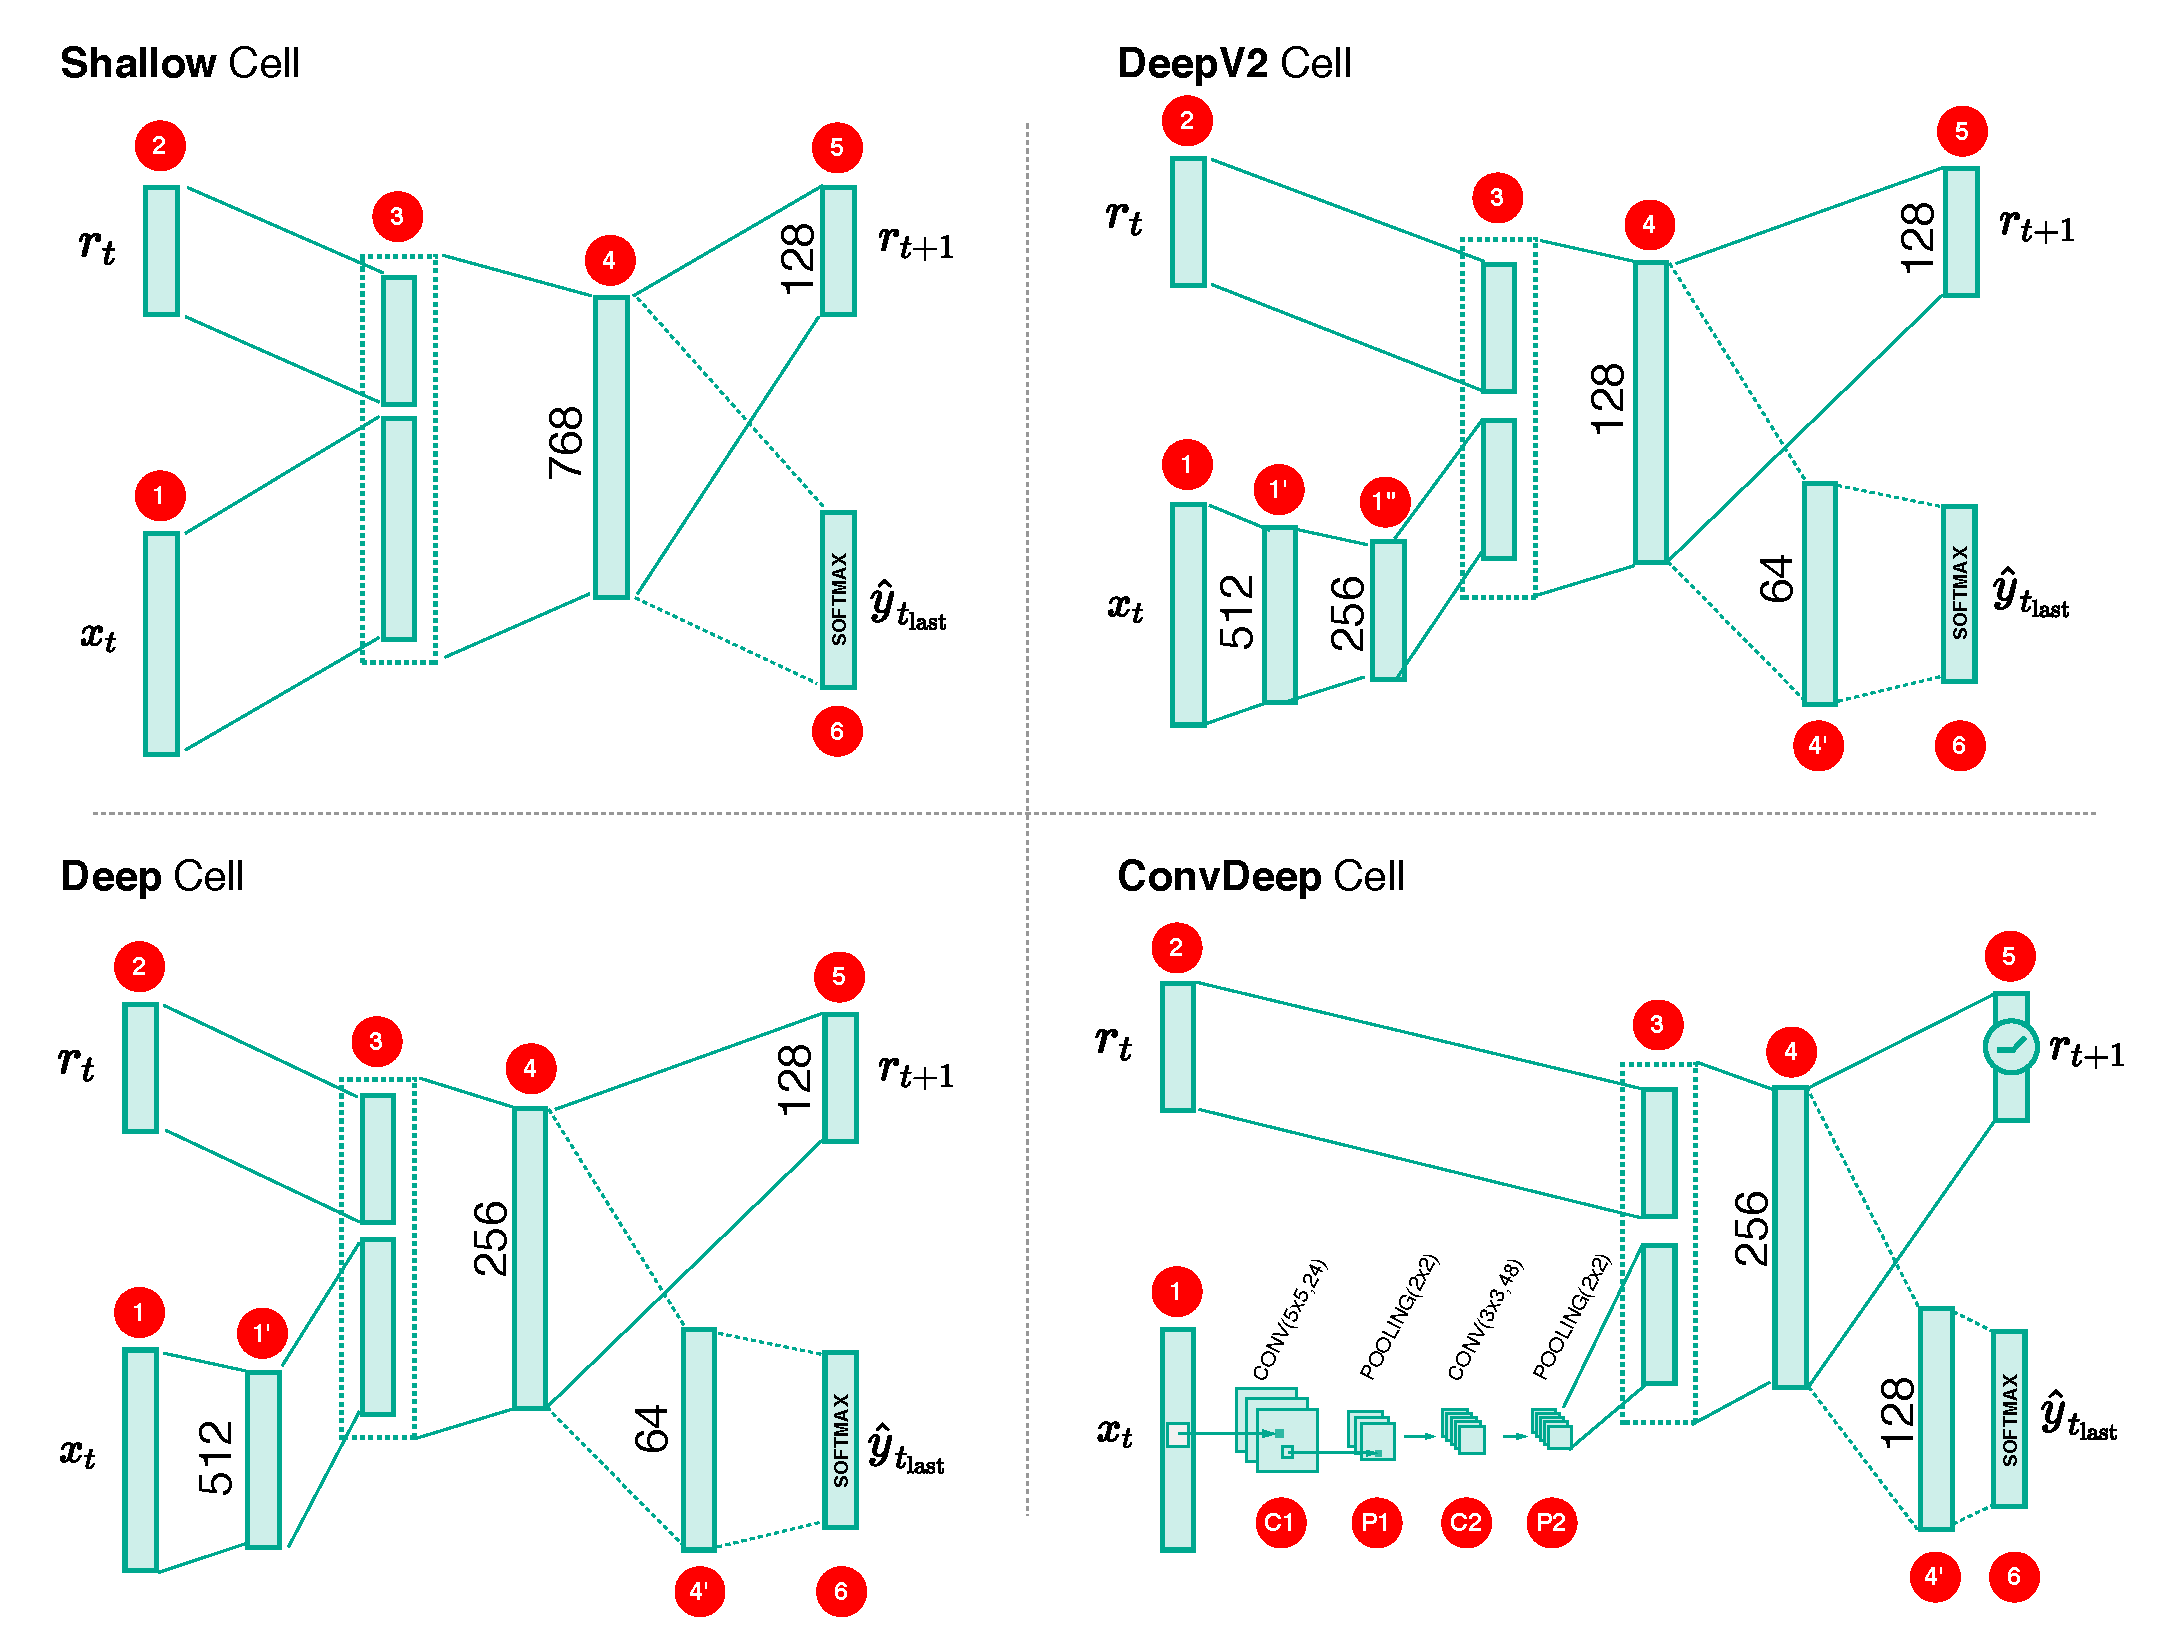
\includegraphics[width=\textwidth]{sketch/neuron_numbers}
%\caption{Number of neurons in each layer for each cell architecture}
%\label{fig:neuron_numbers}
%\end{figure}
%
%
%\begin{itemize}
%	\item \textbf{Shallow Cell} 
%$$\{ n^{(4)}\} = \{ 768 \}$$
%	\item \textbf{Deep Cell} 
%$$\{ n^{(1')}, n^{(4)}, n^{(4')} \} = \{ 512, 256, 64 \}$$
%	\item \textbf{DeepV2 Cell} 
%$$\{ n^{(1')}, n^{(1")}, n^{(4)}, n^{(4')} \} = \{ 512, 256, 128, 64 \}$$
%	\item \textbf{ConvDeep Cell} : 
%\begin{align*}
%	\{ n^{(C1)}, n^{(P1)} \} &= \{ CONV(5\text{x}5, 24), POOL(2\text{x}2) \} \\
%		\{ n^{(C2)}, n^{(P2)} \} &= \{ CONV(3\text{x}3, 48), POOL(2\text{x}2) \} \\
%			\{  n^{(4)}, n^{(4')} \} &= \{ 256, 128 \}
%\end{align*}
%where $CONV(x,y)$ is a convolutional operator with $y$ filters whose kernel size is $\mathbb{R}^{x}$. Similarly, $POOL(x)$ is a pooling operator  with kernel size $\mathbb{R}^{x}$.
%
%
%\end{itemize}
%
%Noting that, $n^{(5)}$ is set at 128 for all architectures and 0 when the sequence length of the problem is 1. $n^{(6)}$ is equal to the number of categories of a problem, for example $n^{(6)} = 10 $ MNIST. Table \ref{tab:variable_architecture} shows the total numbers of variables in details.

%\renewcommand{\arraystretch}{1.2}
%\begin{table}[h]
%\centering
%\begin{tabular}{l|c|c|c|}
%\cline{2-4}
%                                                 & \multicolumn{3}{c|}{\textbf{Sequence Length}} \\ \hline
%\multicolumn{1}{|l|}{\textbf{Cell Architecture}} & 1         & 4         & 7         \\ \hline
%\multicolumn{1}{|l|}{\rnncell{Shallow}}                    & 610570    & 355722    & 291210      \\ \hline
%\multicolumn{1}{|l|}{\rnncell{Deep}}                       & 550346    & 314954    & 271946      \\ \hline
%%\multicolumn{1}{|l|}{\rnncell{DeepV2}}                    & 575050    & 306890    & 263882      \\ \hline
%%\multicolumn{1}{|l|}{\rnncell{ConvDeep}}                   & 647594    & 283178    & 197162      \\ \hline
%\end{tabular}
%\caption{Total variables in each architecture and sequence length}
%\label{tab:variable_architecture}
%\end{table}


 

%\clearpage
\section{Experiment 1 : Sequence Classification}
\label{sec:exp1}

\subsection{Problem Formulation}
We consider this experiment as a preliminary study. Here, we constructed an artificial classification problem using MNIST and FashionMNIST datasets. Each image sample $\x$ is column-wise split into a sequence of non-overlapping $\{ \x_t \}_{t=1}^{T}$. These sequences are used to train RNN classifiers. The RNN classifiers need to summarize information from $\{ \x_t \}_{t=1}^{T}$ to determine what is the class of $\x$.  Using image samples allows us to inspect produced explanations conveniently.

\addfigure{\ref{fig:artificial_problem}} illustrates the setting. As shown in the figure, an MNIST sample $ \patvector{x} \in \mathbb{R}^{28 \times 28}$ is divided to a sequence of $\{ \patvector{x}_t \in   \mathbb{R}^{28 \times 7} \}_{t=1} ^ 4$. At  a time step $t$, $\patvector{x}_t$ is presented to the RNN classifier yielding the recurrent input $\patvector{r}_{t+1}$ for the next step. For the last step $T = 4$, the RNN classifier computes $f(\x) \in \mathbb{R}^{10}$ and the class probabilities accordingly.


 \begin{figure}[!hbt]
		\centering
		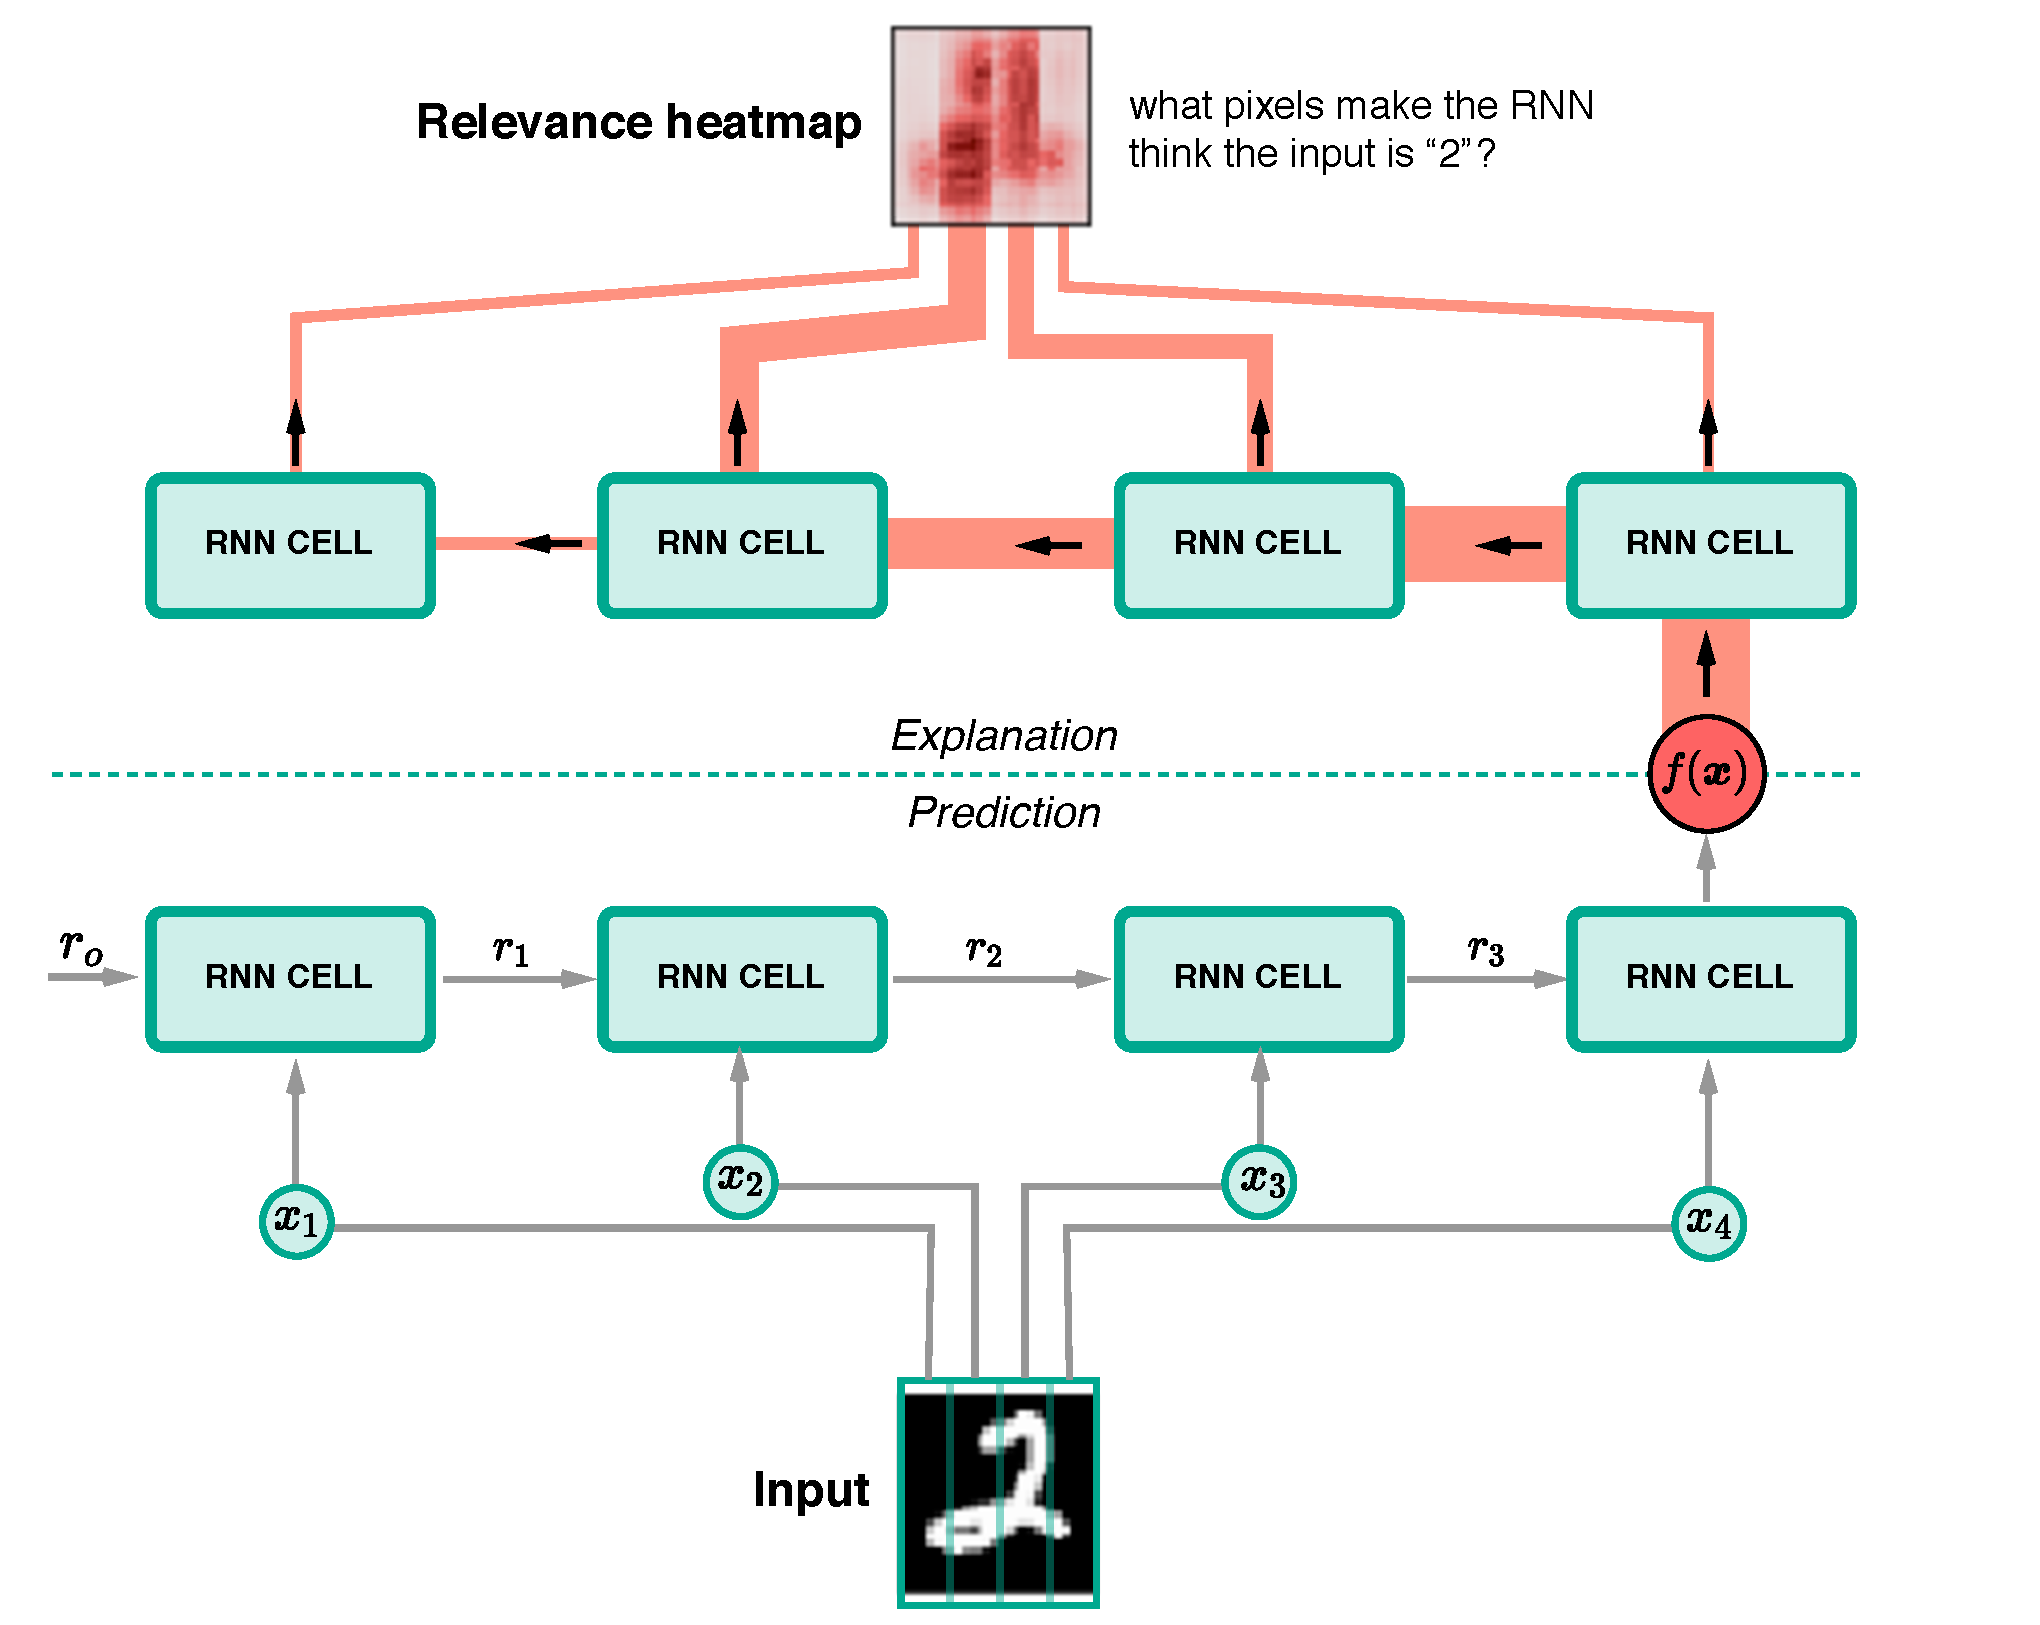
\includegraphics[width=0.8\textwidth]{sketch/artificial_problem_with_rel}
		\caption{Explaining a decision of a RNN classifier.} 
		\label{fig:artificial_problem}
\end{figure}


\begin{figure}[!htb]
\centering

\subfloat[Shallow\label{fig:shallow_arch}]{%
       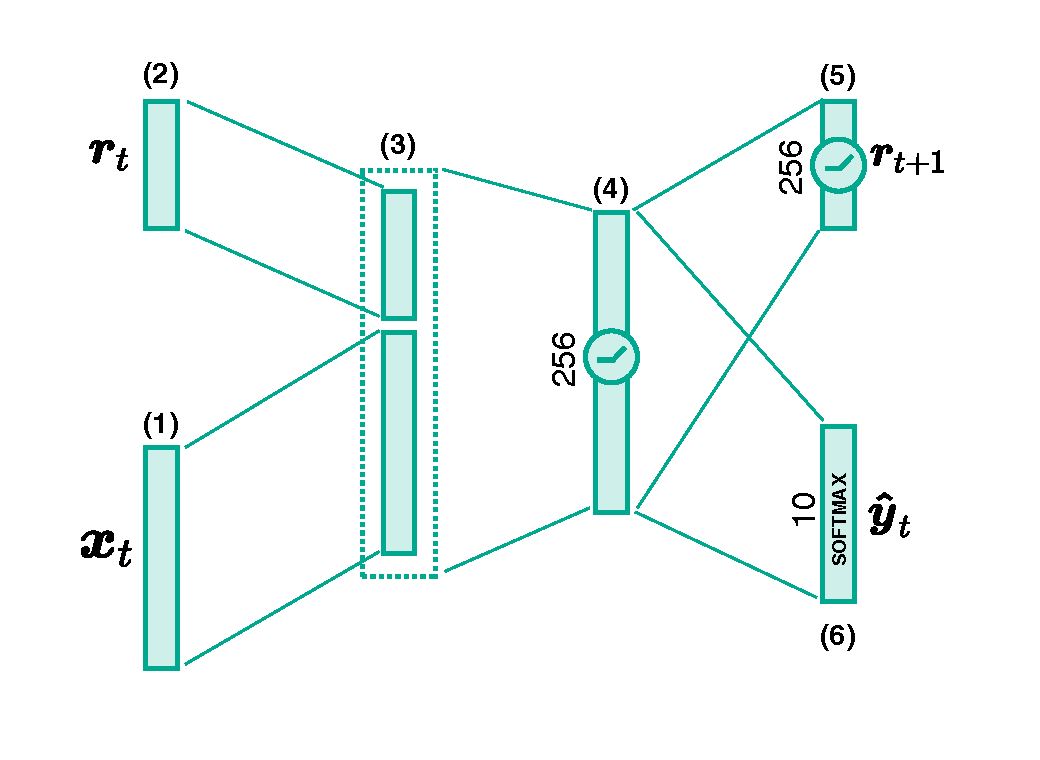
\includegraphics[width=0.48\textwidth]{sketch/shallow_arch}
}
     \hfill
\subfloat[Deep \label{fig:deep_arch}]{%
       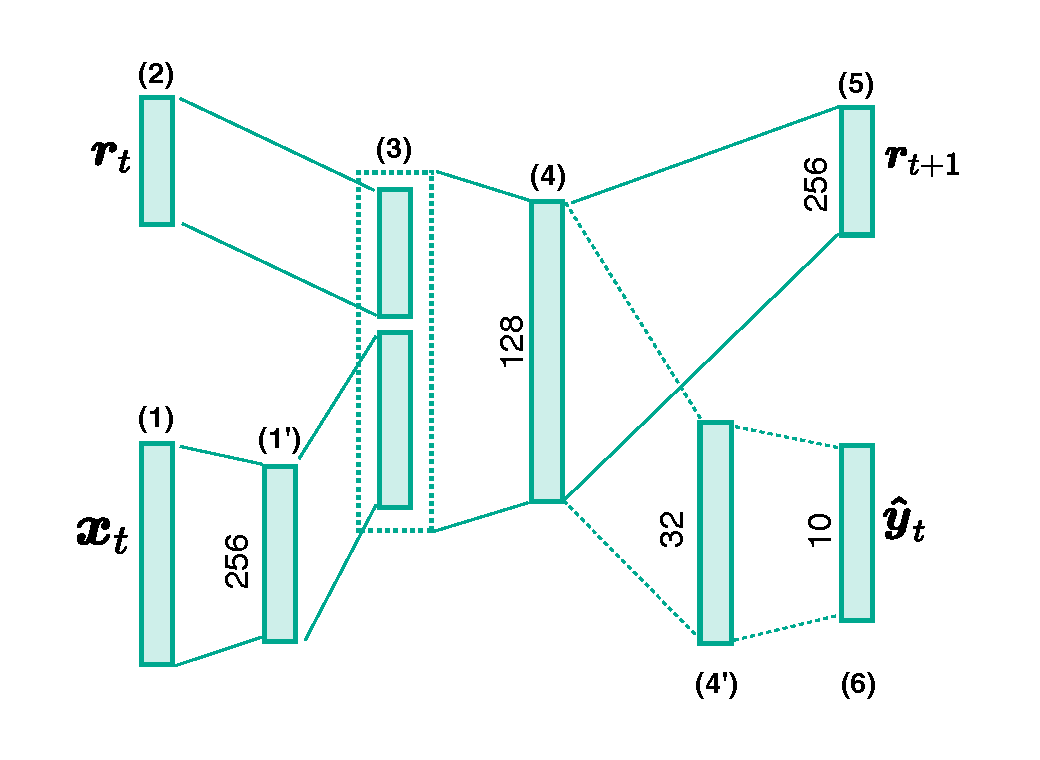
\includegraphics[width=0.48\textwidth]{sketch/deep_arch}
}
\patcaption{Shallow and Deep architectures.}{Numbers of neurons at each layer depicted.}
\end{figure}

In this experiment, we are considering two RNN architectures, namely

\begin{enumerate}
	\item \textbf{Shallow architecture}  \ \ \ as shown in \addfigure{\ref{fig:shallow_arch}}, for a time step $t$, the \rnncell{Shallow} architecture first concatenates the input $\patvector{x}_t$  and the recurrent input $\patvector{r}_t$ at the layer \circled{3} as one vector before computing activations of the layer \circled{4}, denoted as $\patvector{a}_t^{(4)}$. Then,  the next recurrent input $\patvector{r}_{t+1}$ \circled{5}	 is derived from $\patvector{a}_t^{(4)}$. In the last step $T$, $f(\x)$ is computed from $\patvector{a}^{(4)}_{T}$ and supplied to the softmax function to calculate the class probabilities $\patvector{\hat{y}}$. 
		
Because the activations coming to the layer \circled{4} are from different domains: more precisely, $x_{t,i} \in [-1, 1]$ and $r_{t,j} \in [0, \infty) $, a special propagation rule is required in order to apply DTD. Particularly, the relevance score is needed to be propagated to those sources as follows
% For neuron $i$ in $\x_t$ and neuron $j$ in $\patvector{r}_t$ respectively that connect to neuron $k$ in \circled{4}, their relevance are calculated as follow
		
\begin{align*}
	R_{t, i} &= \sum_k \frac{(x_{t, i} w_{ik} - l_i w_{ik}^+ - h_i w_{ik}^-) R_{t,k}}{z_{t,k}} \\	
     R_{t, j} &= \sum_k \frac{r_{t, j} w_{jk}^+ R_{t,k}}{z_{t,k}},
\end{align*}
where $z_{t,k} = \sum_j r_{t,j} w_{jk}^+ + \sum_i x_{t,i} w_{ik} - l_i w_{ik}^+ - h_i w_{ik}^-$ is the normalization term with $w_{jk}^+ = \max(0, w_{jk})$, and $w_{jk}^- = \min(0, w_{jk})$.

	\item \textbf{Deep architecture} \ \ \ \addfigure{\ref{fig:deep_arch}} illustrates the configuration of this architecture. Unlike the Shallow architecture, the Deep cell has 2 more layers, namely the \circled{1'} and \circled{4'} layers.  The improvement would allow the \circled{1'} layer to learn representations from input properly and the \circled{4} layer to efficiently combine information from the past and current input. 
\end{enumerate}

\renewcommand{\arraystretch}{1.5}
\begin{table}[h]
\centering
\begin{tabular}{cc|c|c|}
\cline{3-4}
& & \multicolumn{2}{c|}{\textbf{No. trainable variables}}                                                                \\ \hline
\multicolumn{1}{|c|}{\textbf{T}}               & \multicolumn{1}{c|}{\textbf{Dim. of $\x_t$}} & \multicolumn{1}{c|}{\textbf{Shallow}} & \multicolumn{1}{c|}{\textbf{Deep}}  \\ \hline
\multicolumn{1}{|c|}{1} & $\mathbb{R}^{28 \times 28}$ & 269,322  &  271,338 \\
\multicolumn{1}{|c|}{4} & $\mathbb{R}^{28  \times  7}$ & 184,330 & 153,578 \\
\multicolumn{1}{|c|}{7} & $\mathbb{R}^{28  \times  4}$ & 162,826 & 132,074 \\ \hline

\end{tabular}
\caption{Dimensions of $\patvector{x}_t$ and number of trainable variables in each architecture on different sequence lengths $T=\{1, 4, 7\}$.}
\label{tab:seq-length}
\end{table}
\renewcommand{\arraystretch}{1}




We experimented this sequence classification using sequence lengths $T = \{1, 4, 7\}$.  Table \ref{tab:seq-length} shows the dimensions of $\patvector{x}_t$ for different sequence lengths as well as the number of trainable variables in each architecture. To simplify the writing, we are going to use a convention \textit{\rnncellseq{ARCHITECTURE}{T}} to denote the \textit{ARCHITECTURE} model trained on the sequence length \textit{T}. For example, \rnncellseq{Deep}{7} refers to the Deep architecture trained on $\{ \x_t \in \mathbb{R}^{28 \times 4} \}_{t=1}^{7}$.

\subsection{Result}
\label{sec:exp1_result}

\renewcommand{\arraystretch}{1.5}
\begin{table}[]
\centering
\begin{tabular}{cc|c|c|c|}
\cline{2-5}
& \multicolumn{2}{|c|}{\textbf{MNIST}} & \multicolumn{2}{|c|}{\textbf{FashionMNIST}} \\ \hline
\multicolumn{1}{|c|}{$T$}   & \multicolumn{1}{c|}{\textbf{Shallow}} & \multicolumn{1}{c|}{\textbf{Deep}} & \multicolumn{1}{c|}{\textbf{Shallow}} & \multicolumn{1}{c|}{\textbf{Deep}} \\ \hline
\multicolumn{1}{|c|}{1} & 98.11\%   & 98.22\% & 87.93\%  & 89.14\%                           \\
\multicolumn{1}{|c|}{4} & 98.56\% & 98.63\%  & 89.04\%  & 89.43\%                            \\
\multicolumn{1}{|c|}{7} & 98.66\%  & 98.68\% & 89.28\%  & 88.96\%  \\ \hline
\end{tabular}
\patcaption{Sequence classification accuracies from the Shallow and Deep architecture trained with different sequence lengths.}{The accuracies are computed from the test set.}
\label{tab:mnist_model_acc}
\end{table}
\renewcommand{\arraystretch}{1}



 \begin{figure}[!htb]
\centering
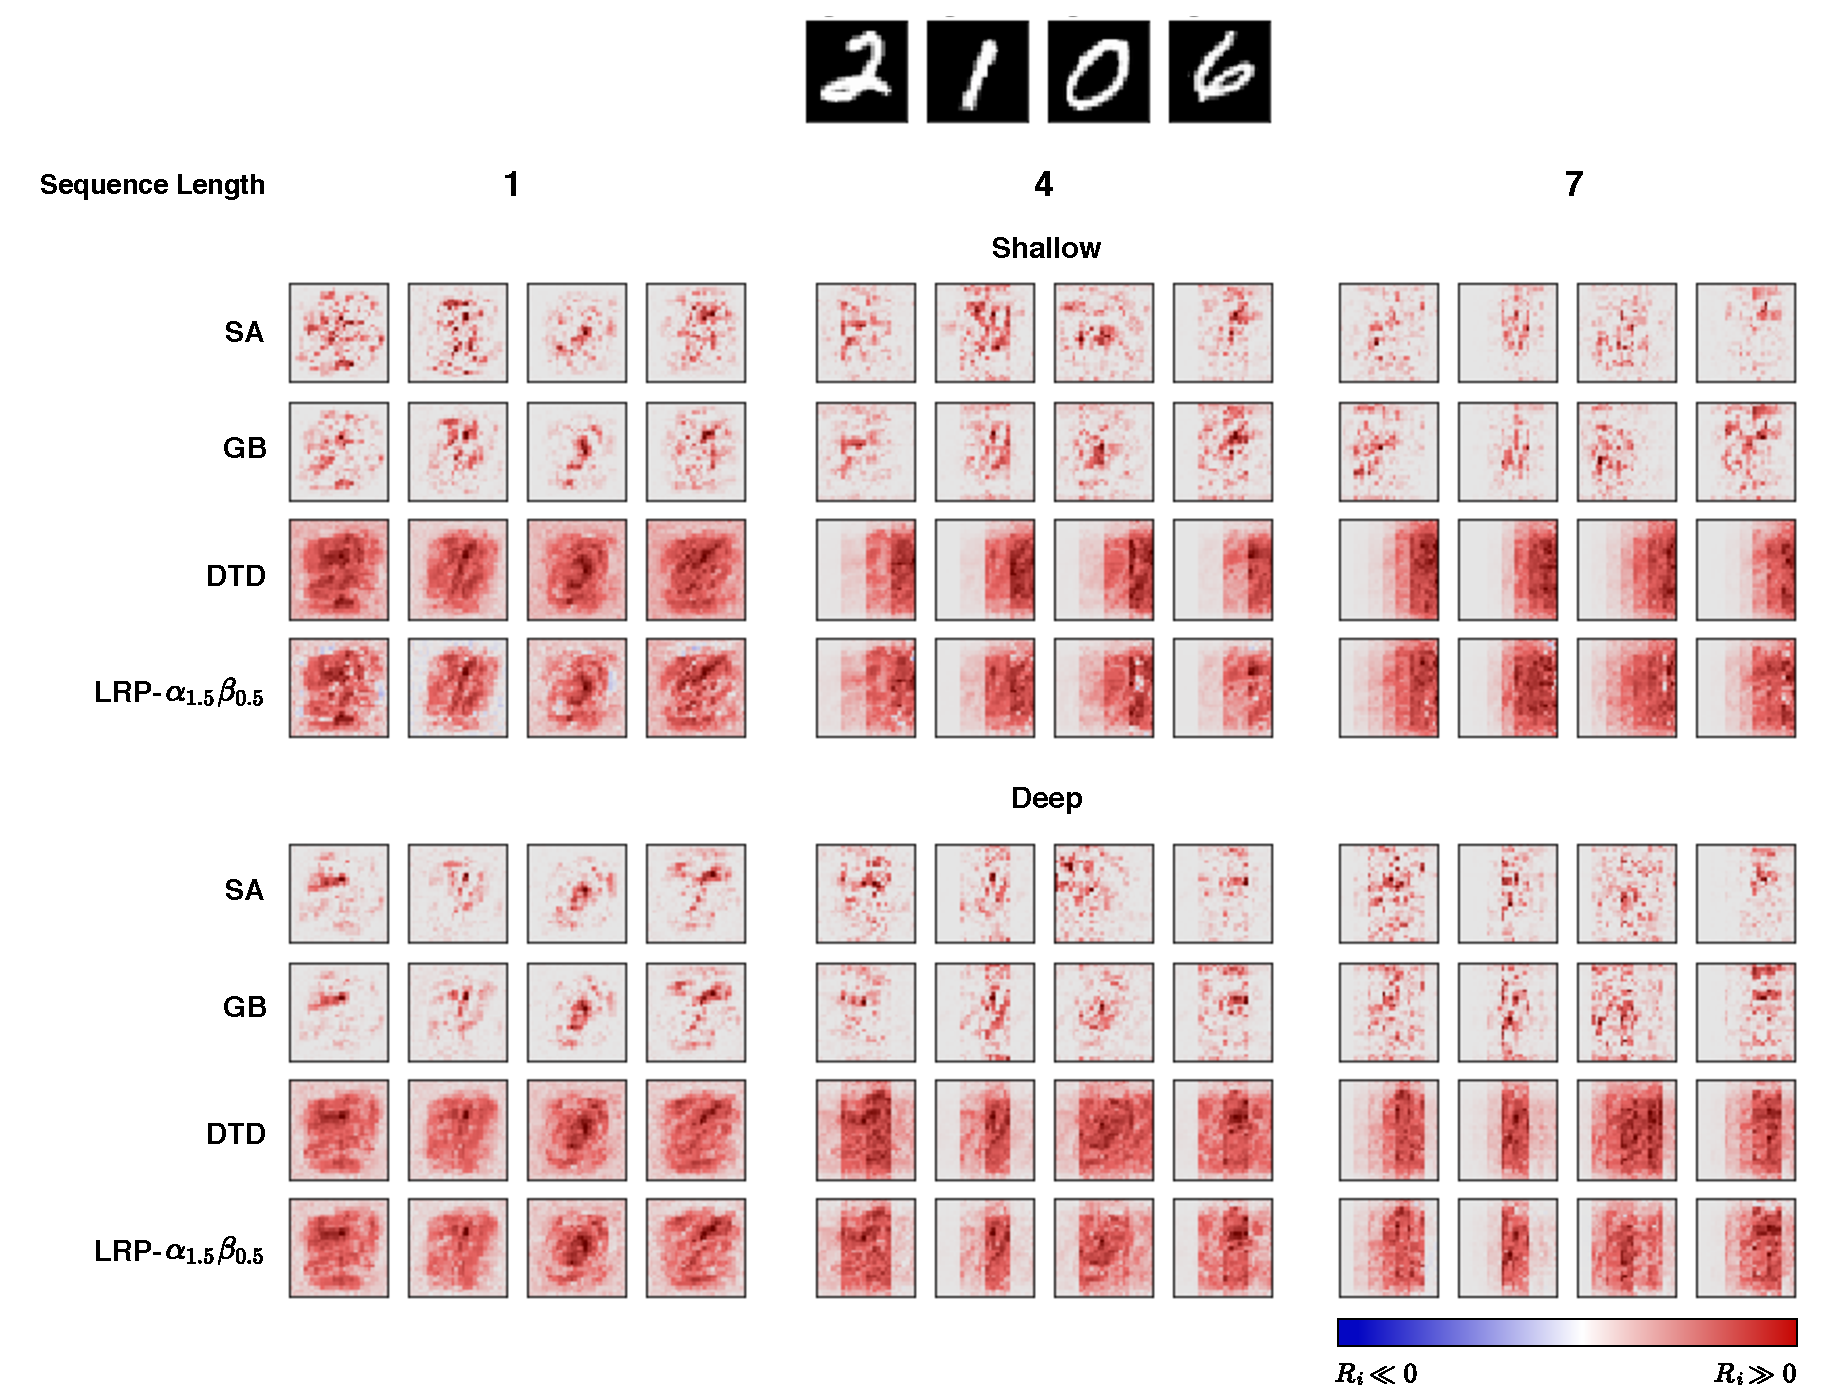
\includegraphics[width=0.8\textwidth]{sketch/mnist_experiment}
\patcaption{Relevance heatmaps from different explanation techniques applied to the Shallow and Deep architectures trained on MNIST with different sequence lengths.}{\heatmapscaleexplain }
\label{fig:mnist_experiment}
\end{figure}


Table \ref{tab:mnist_model_acc} summarizes accuracy of the trained models. Both Shallow and Deep architectures have comparable accuracy; hence their explanations can be compared. \addfigure{\ref{fig:mnist_experiment}} shows relevance heatmaps from the two architectures trained on MNIST.  We can observe the similar characteristics of each explanation technique as in \addfigure{\ref{fig:lenet_heatmaps}}. In particular, SA and GB explanations are sparse, while the ones from DTD and $\lrpp$ are more diffuse throughout $\x$. 

\rnncellseq{Shallow}{1}  and \rnncellseq{Deep}{1} have similar relevance heatmaps regardless of explanation methods.  However, as the sequence length increased, \rnncellseq{Shallow}{4,7} and  \rnncellseq{Deep}{4,7} start producing  different relevance heatmaps when being explained by DTD and $\lrpp$.  In particular,  the explanations from \rnncellseq{Shallow}{4,7}  are mainly concentrated on the right part. This area corresponds to input of the last time steps. On the other hand,  the explanations from \rnncellseq{Deep}{4,7} are proportionally  highlighted around the content area of $\x$. We do not observe this effect from SA and GB.


 \begin{figure}[!htb]
\centering
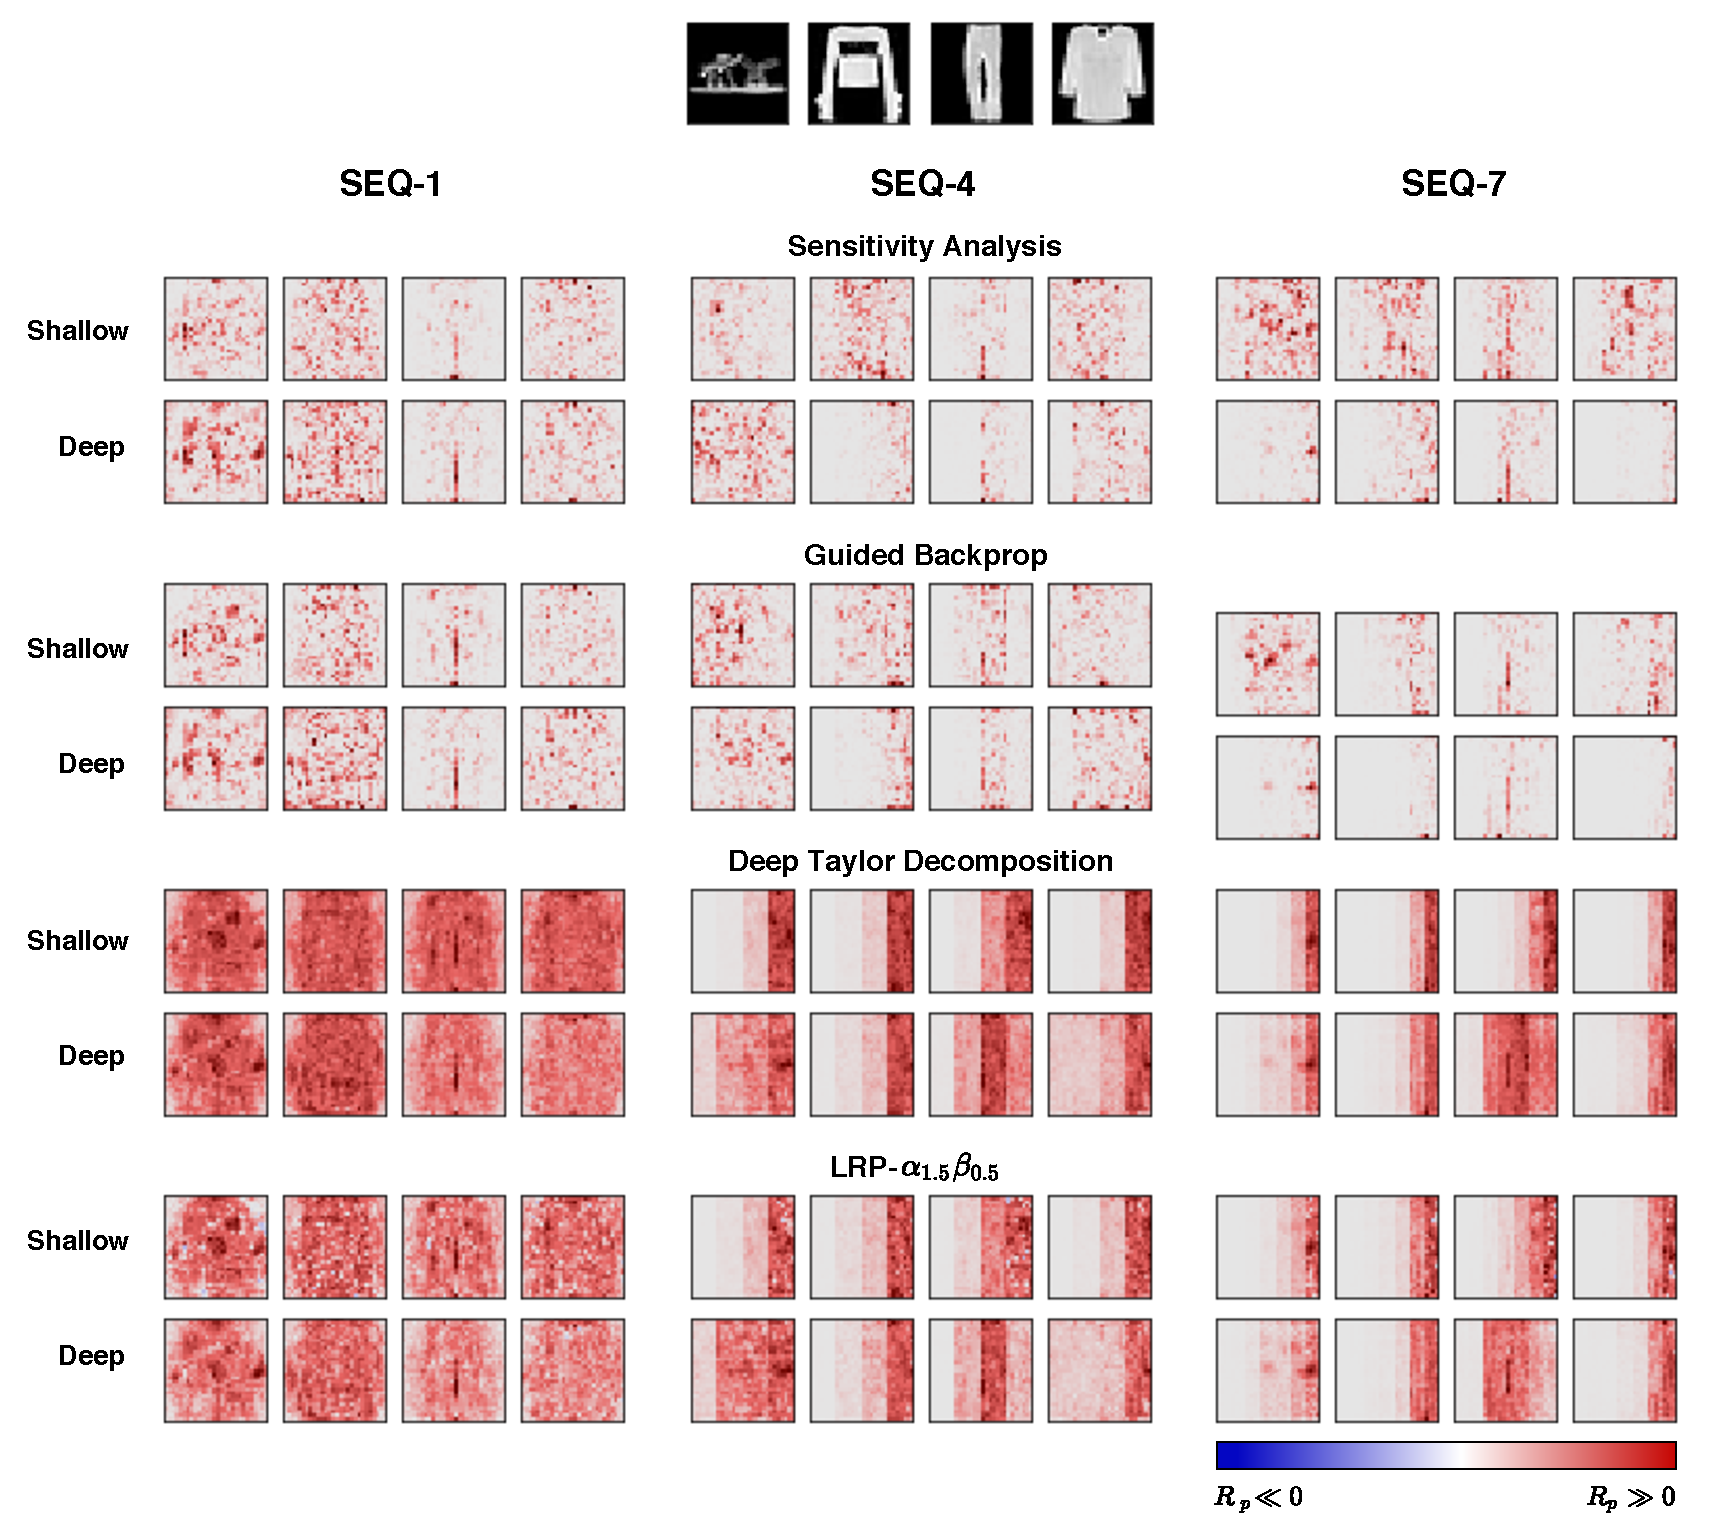
\includegraphics[width=0.8\textwidth]{sketch/fashion_mnist_experiment}
\patcaption{Relevance heatmaps from different explanation techniques applied to the Shallow and Deep architecture trained on FashionMNIST with different sequence lengths.}{\heatmapscaleexplain}
\label{fig:fashion_mnist_experiment}
\end{figure}

Relevance heatmaps of the Shallow and Deep architectures trained on  FashionMNIST  are shown on \addfigure{\ref{fig:fashion_mnist_experiment}}. Similar to the ones from MNIST. We do not see any remarkable difference on SA and GB heatmaps between the two architectures although \rnncellseq{Deep}{4,7} produces slightly more sparse heatmaps than \rnncellseq{Shallow}{4,7}. However, the wrong concentration issue of DTD and LRP seems to appear on the heatmaps from both \rnncellseq{Shallow}{4,7} and \rnncellseq{Deep}{4,7}. Nevertheless, we can still observe appropriately allocated relevance from \rnncellseq{Deep}{4,7} on some samples. For example, consider the trouser sample. We can see  that \rnncellseq{Deep}{4,7} manage to distribute high relevance scores to the area of the trouser.  We suspect that the Deep architecture is not capable enough to learn proper representations from FashionMNIST samples in which many visual features are shared between classes. Consider \textit{Sneaker} and \textit{Ankle Boot} samples in \addfigure{\ref{fig:fmnist_similar_samples}}. One can see that  their front parts are similar and only the heel part that determines the difference between the two categories. This evidence suggests that it is preferable to employ more robust feature extractor layers, such as convolution and pooling layers, instead of using only the fully-connected ones.

 \begin{figure}[!htb]
\centering
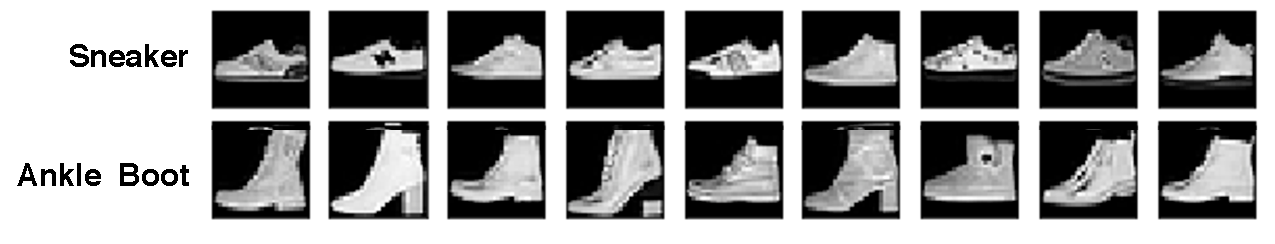
\includegraphics[width=0.8\textwidth]{sketch/fmnist_similar_samples}
\patcaption{Sneaker and Ankle Boot samples in FashionMNIST.}{}
\label{fig:fmnist_similar_samples}
\end{figure}

 \begin{figure}[!htb]
\centering
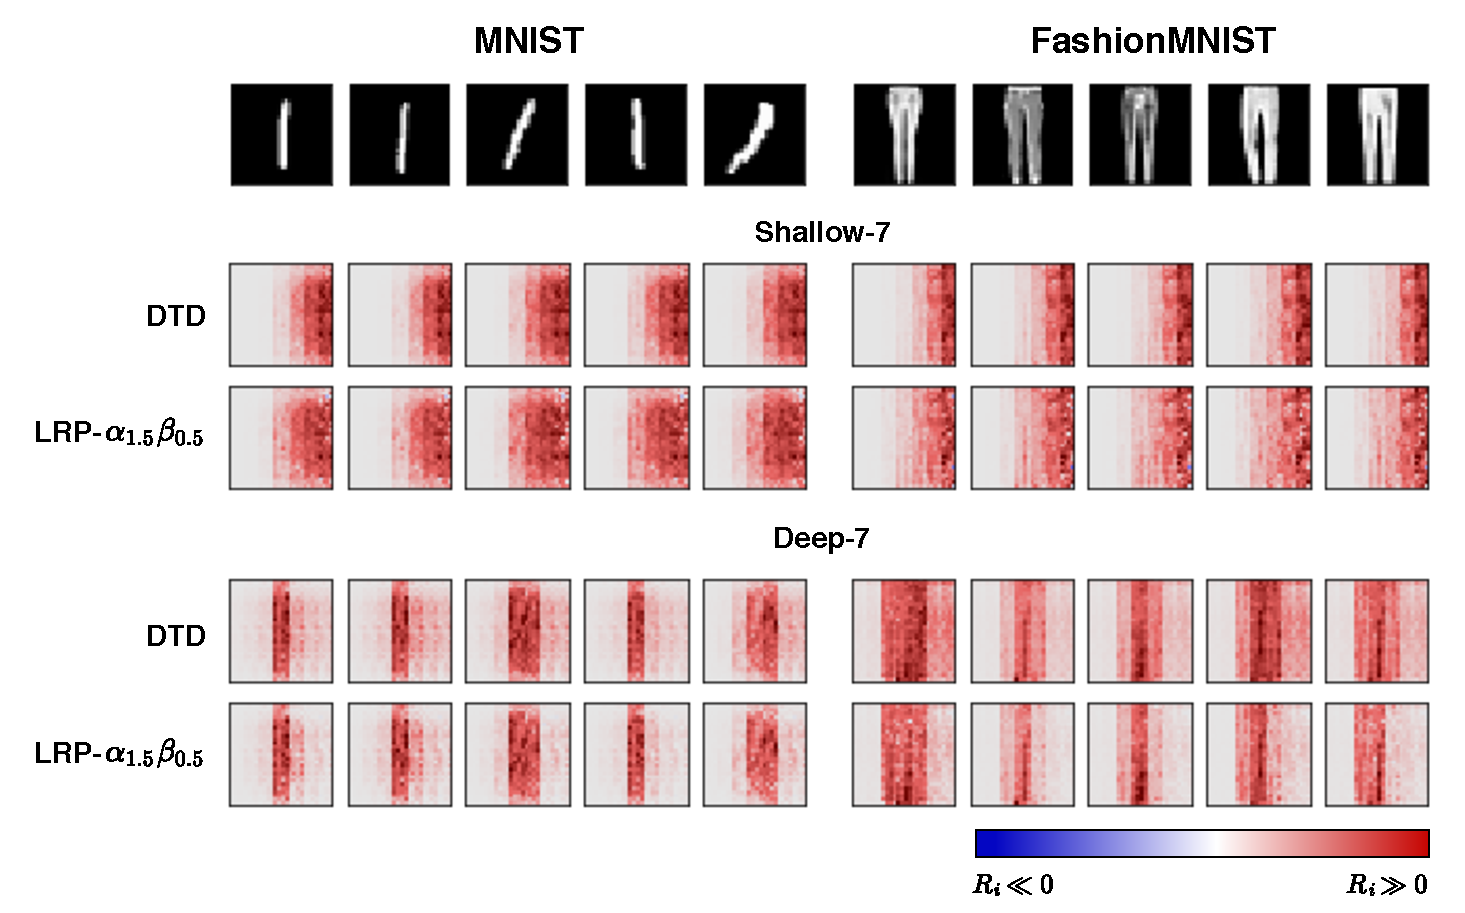
\includegraphics[width=0.8\textwidth]{sketch/class_1_comparison}
\patcaption{Relevance heatmaps of MNIST \textit{Digit 1} and FashionMNIST \textit{Trouser} samples from \rnncellseq{Shallow}{7} and \rnncellseq{Deep}{7} explained by DTD and $\lrpp$ methods.}{\heatmapscaleexplain }
\label{fig:class_1_comparison}
\end{figure}

\addfigure{\ref{fig:class_1_comparison}} presents explanations of MNIST \textit{Digit 1} and FashionMNIST \textit{Trouser} samples from \rnncellseq{Shallow}{7} and \rnncellseq{Deep}{7}. These samples are chosen to emphasize the impact of RNN architecture on DTD and LRP explanations. As can be seen from the figure, these samples have $\x_{t'}$ containing the actual content primarily locating around the middle of the sequence. Hence, suitable relevance heatmaps should be highlighted at $\x_{t'}$ and possibly its neighbors.  As expected, we can see that \rnncellseq{Deep}{7} produces sound explanations in which the heatmaps have high-intensity value where $\x_{t'}$ approximately locates, while \rnncellseq{Shallow}{7} mainly assigns relevance quantities to $\x_{t}$ for $t \approx T$. 

\addfigure{\ref{fig:exp1_dist_plot}} further shows quantitive evidence of this improper propagation issue of DTD and LRP. Here, distributions of relevance scores derived from the methods on \rnncellseq{Shallow}{7} and \rnncellseq{Deep}{7} are plotted across time step $t = \{ 1, \dots, 7 \}$. The distributions are computed from all test samples in MNIST \textit{Digit 1} and FashionMNIST \textit{Trouser} respectively. The plots also include distribution of pixel  values.  We can see that the distributions of relevance scores from \rnncellseq{Deep}{7} align with the distributions of pixel values , while  the ones from \rnncellseq{Shallow}{7}  diverge by a significant margin. Approximately, \rnncellseq{Shallow}{7} distributes more than 90\% of relevance scores to the last three steps, namely $\x_5$, $\x_6$ and $\x_7$.


 \begin{figure}[!htb]
\centering
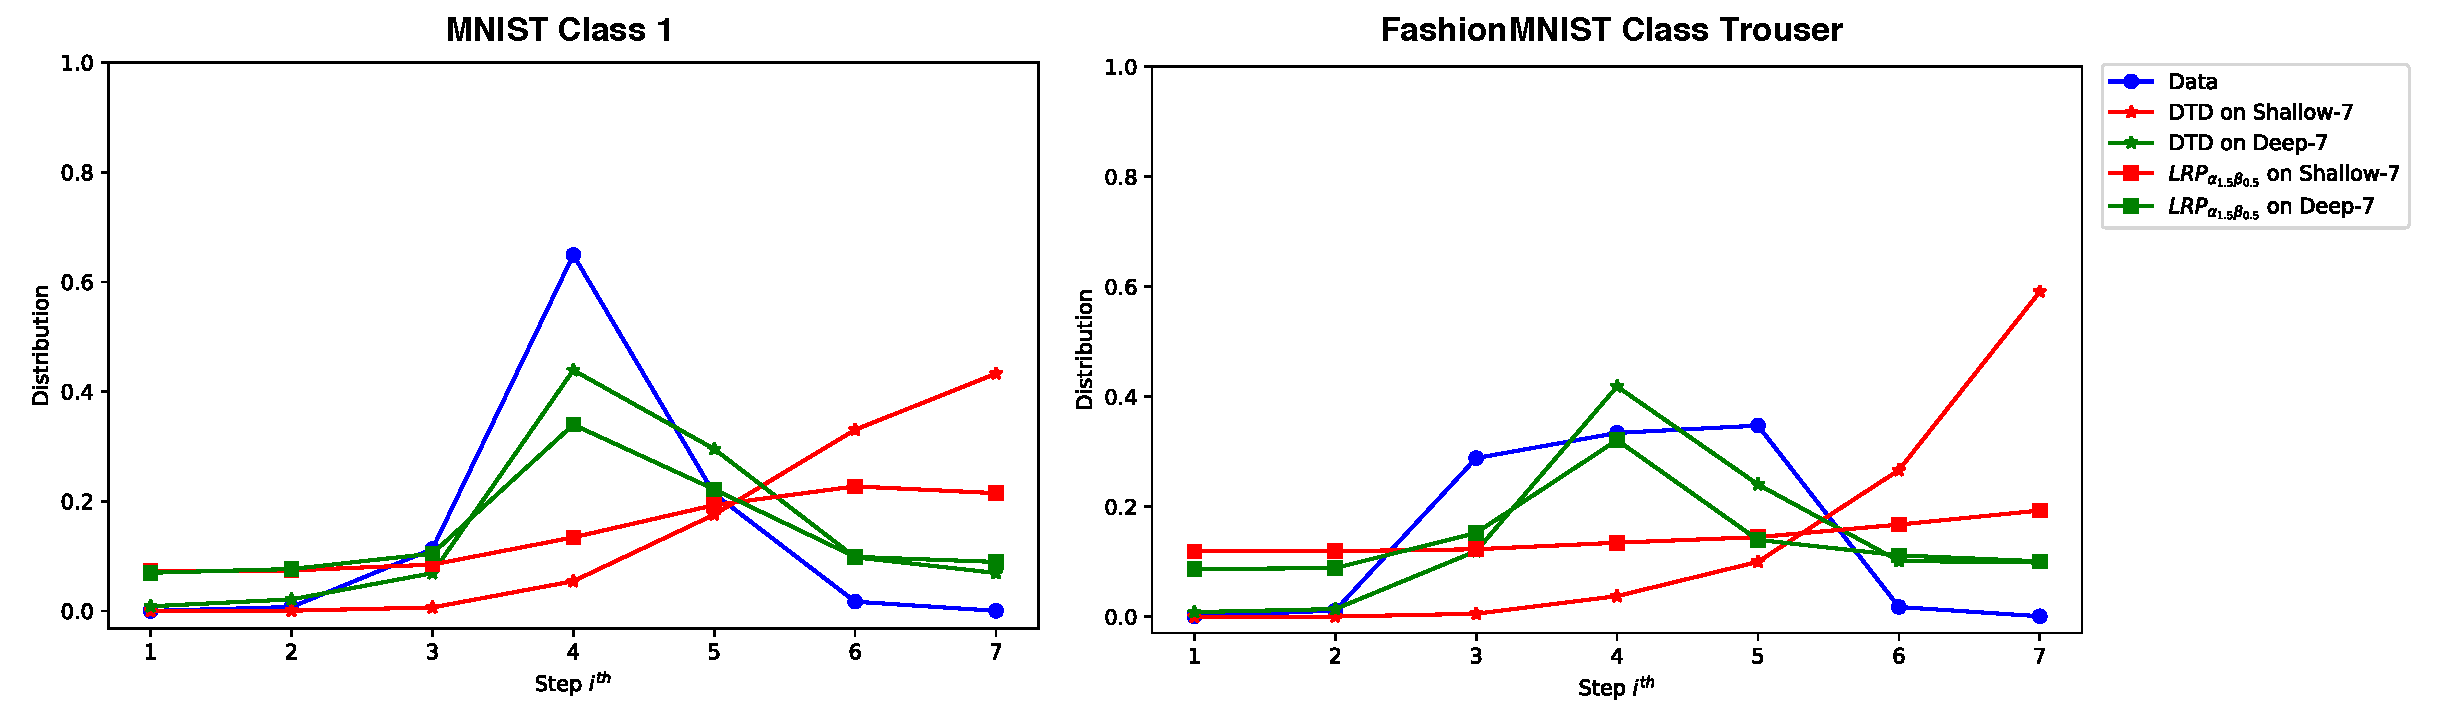
\includegraphics[width=\textwidth]{sketch/exp1_dist_plot}
\caption{Distributions of pixel intensities and relevance quantities of MNIST \textit{Digit 1} and FashionMNIST \textit{Trouser}  test population from \rnncellseq{Shallow}{7} and \rnncellseq{Deep}{7} explained by DTD and $\lrpp$ methods. The distributions of relevance quantities from \rnncellseq{Shallow}{7}  are plotted in red, the ones from \rnncellseq{Deep}{7} are plotted in green, and the distribution of pixel intensities are plotted in blue.} 
\label{fig:exp1_dist_plot}
\end{figure}

\subsection{Summary}
The results of this preliminary experiment strongly support our hypothesis that the structure of RNNs could have an impact on the quality of  explanation.  In particular,  as presented in \addfigure{\ref{fig:class_1_comparison}} and \addfigure{\ref{fig:exp1_dist_plot}}, the quality of DTD and $\lrpp$ explanations is significantly influenced by the architecture. In contrast, we do not see such notable effect on SA and GB method.  In the following, we are going to discuss a similar experiment that is designed in a more constructive way such that we can methodologically evaluate the impact of RNN architecture on explanation.


\section{Experiment 2 : Majority Sample Sequence Classification} \label{sec:exp2}
   
 \begin{figure}[!htb]
\centering
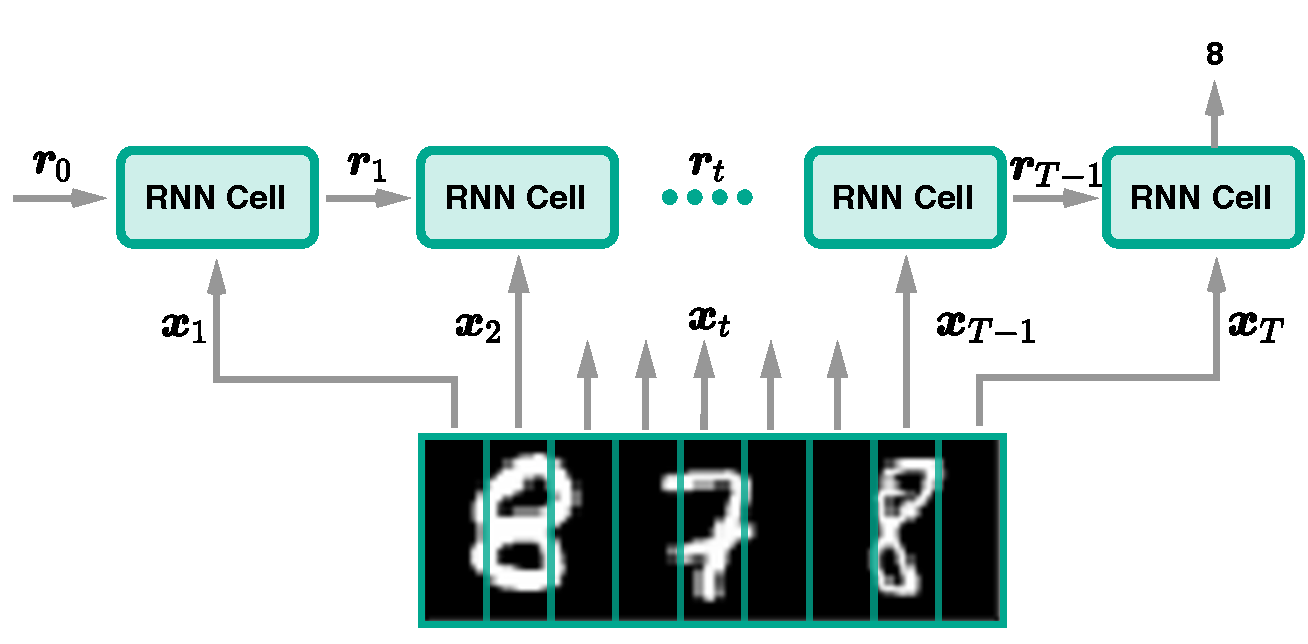
\includegraphics[width=0.8\textwidth]{sketch/artificial_problem_3digits}
\caption{Majority Sample Sequence Classification (MAJ) problem.} 
\label{fig:artificial_problem_3digits}
\end{figure}

\subsection{Problem Formulation} \label{sec:exp2_prob_formulate}
When a neural network (NN) is trained, one can apply explantation techniques to the model to get explanations of the outputs.  The explanation of a sample $\x$ indicates the contribution of features in $x$ that the trained network relies on to perform the objective task.  Therefore, one needs to know the ground truth where these latent features are to methodologically evaluate the explainability of the model.  However, this knowledge is not trivially available because we do not explicitly tell the NN which features of $\x$ to use when marking predictions.

% in is a result from the training process that we, in fact, seek to understand in the first place.

To alleviate this challenge, we propose another artificial classification problem where a RNN is trained to classify  the majority group in a sequence $\x = \{ \x_t \}_{t=1}^{T}$. Consider  the MNIST dataset. The input $\x$ is constructed as follows: for each original MNIST sample $\widetilde{\x} \in \mathbb{R}^{28 \times 28}$, we randomly selected two additional samples: one from the same class of $\widetilde{\x}$ and the other one from a different class. Then, these three samples are concatenated in a random order yielding a sample $\x \in \mathbb{R}^{28 \times 84}$.  \addfigure{\ref{fig:artificial_problem_3digits}} illustrates the data construction and the classification objective. Given $\x = \{ 8, 7, 8\}$, the classification target is ``8".  We call this problem as MNIST-MAJ when $\x$ is constructed from MNIST samples and the same for FashionMNIST-MAJ. With this construction, we can perform quantitative evaluations by measuring relevance scores allocated to $28\times28$ blocks that belong to the majority group.
%
%Because we already know blocks of digit/item that belong to the majority group from the construction,  we can then use this information to  quantitively evaluate  explanation quality  of each RNN.


As discussed in the previous experiment, only some DTD and $\lrpp$ explanations from the Deep architecture on FashionMNIST were sound, this suggests that the architecture does not have enough capability to extract proper representations from FashionMNIST samples, causing the incorrect propagation issue. Hence, apart from the Shallow and Deep architectures, we are going to  introduce another two architectures, namely DeepV2 and ConvDeep. The DeepV2 architecture has one more layer after the first fully-connected layer than the Deep cell. On the other hand, the ConvDeep architecture instead replaces the first layer with  a sequence of convolutional and pooling layers. \addfigure{\ref{fig:deep_conv_arch}} shows details of the new architectures.



%\subsection{Setting}
%Two variations of \rnncell{Deep} cell are also experimented, namely \rnncell{DeepV2} and \rnncell{ConvDeep}, shown on \addfigure{\ref{fig:deep_conv_arch}}. The former has one additional layer \circled{1"} with dropout regularization  between \circled{1'}. On the other hand, the latter replaces fully connected layers between \circled{1} and \circled{3} with 2 convolutional and max pooling layers, \Big[\circled{C1}, \circled{P1}\Big] and \Big[\circled{C2},\circled{P2}\Big].

\begin{figure}[!htb]
\centering

\subfloat[DeepV2\label{fig:deep_4l_network}]{%
       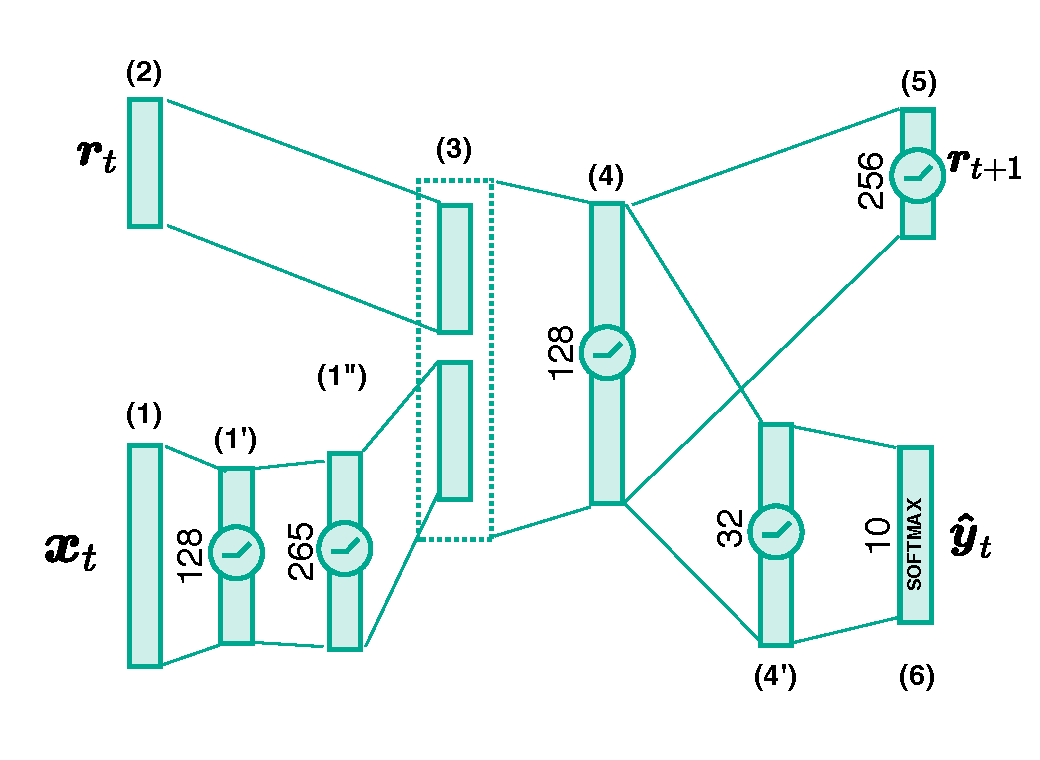
\includegraphics[width=0.48\textwidth]{sketch/deep_v2_arch}
     }
     \hfill
     \subfloat[ConvDeep\label{fig:convdeep_4l_network}]{%
       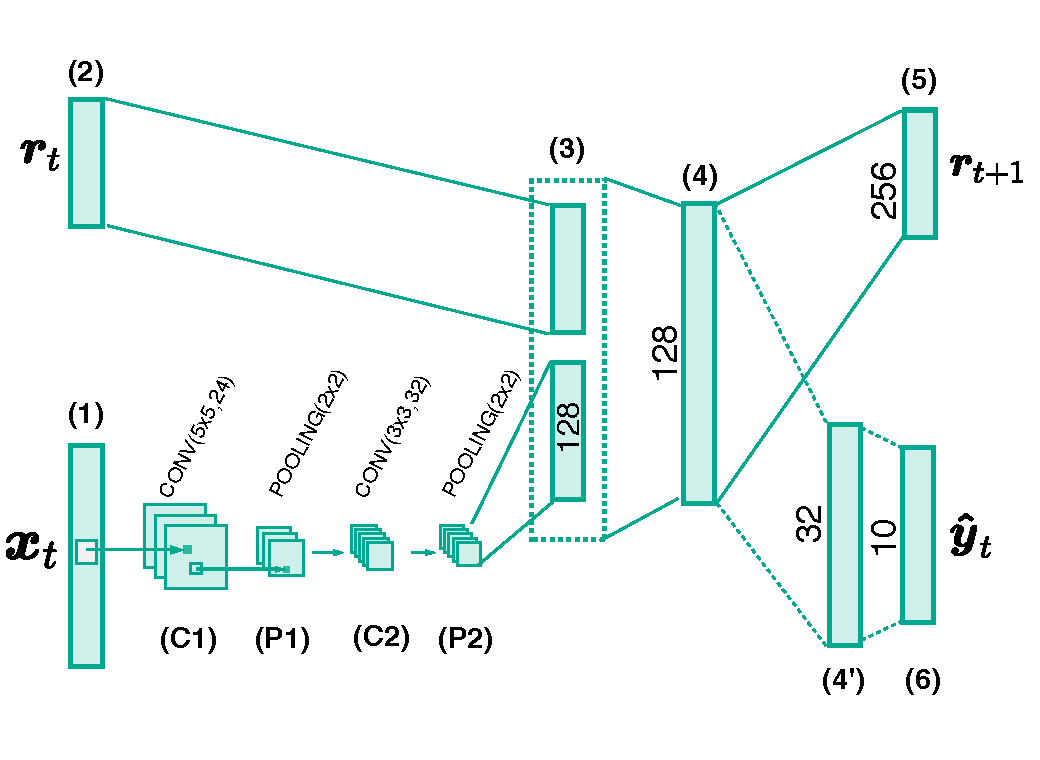
\includegraphics[width=0.48\textwidth]{sketch/convdeep_arch}
     }

\patcaption{DeepV2 and ConvDeep architecture.}{Numbers of neurons at each layer depicted.}
\label{fig:deep_conv_arch}
\end{figure}

Lastly, despite the fact that  our implementation is ready to apply on different sequence lengths,  we experimented with only a sequence length $T=12$ or $\x = \{ \x_t \in \mathbb{R}^{28 \times 7}\}_{t=1}^{12}$. This is mainly due to the limited computational resources and the time constraint we had. Consequently, we are going to write only the name of architecture without explicitly stating the sequence length as we previously did.  We used the same training configuration as described in Section \ref{sec:setup} to train models for this experiment.


\subsection{Evaluation Methodology}
\label{sec:evaluation_med}
From the problem construction, we know that relevance quantities should  be primarily assigned to $28\times28$ blocks associating to the majority group. This construction directly enables us to visually examine the quality of explanations as well as performing quantitative evaluations.  In particular, for qualitative evaluations (i.e. visual inspections), we constructed the training and testing sets based on the original training and testing splits that \citet{LeCunMNISThandwrittendigit2010} and \citet{XiaoFashionMNISTNovelImage2017} provided. 

\subsubsection{Quantitative Evaluation}
A straightforward way to quantify the explanation quality is to calculate the percentage of relevance scores propagated to the blocks of the majority group. However, this measurement has a shortcoming where a architecture can achieve a high percentage if it simply distributes all relevance scores to only one of the correct blocks. Hence, we instead propose to use the \textit{cosine similarity},


\begin{align*}
\cos (\patvector{m}, \patvector{\upsilon}) = \frac{ \patvector{m}^T \patvector{\upsilon}}{ \| \patvector{m}  \| \|\patvector{\upsilon}   \|}	
\end{align*}

The cosine similarity is computed from  a  binary  vector $\patvector{m} \in \{(1,1,0), (1,0,1), (0, 1, 1) \} $  whose entries indicate whether the corresponding $28\times28$ block belongs to the majority group, and a vector $\patvector{\upsilon} \in \mathbb{R}^3$ containing the percentage of  relevance scores distributed to each block. 


As illustrated in \addfigure{\ref{fig:quantitative_evaluation}}, the percentage of correctly distributed relevance scores can be significantly high although the relevance heatmap does not show any highlight at the leftmost block of ``0". Therefore, using cosine similarity is more reasonable. In fact, the propagation needs to be equally balanced between the two blocks in order to achieve the highest score (i.e. 1). 

For $\lrpp$ heatmaps, we ignore negative relevance and set it to zero before computing the cosine similarity.

\begin{figure}[!htb]
\centering
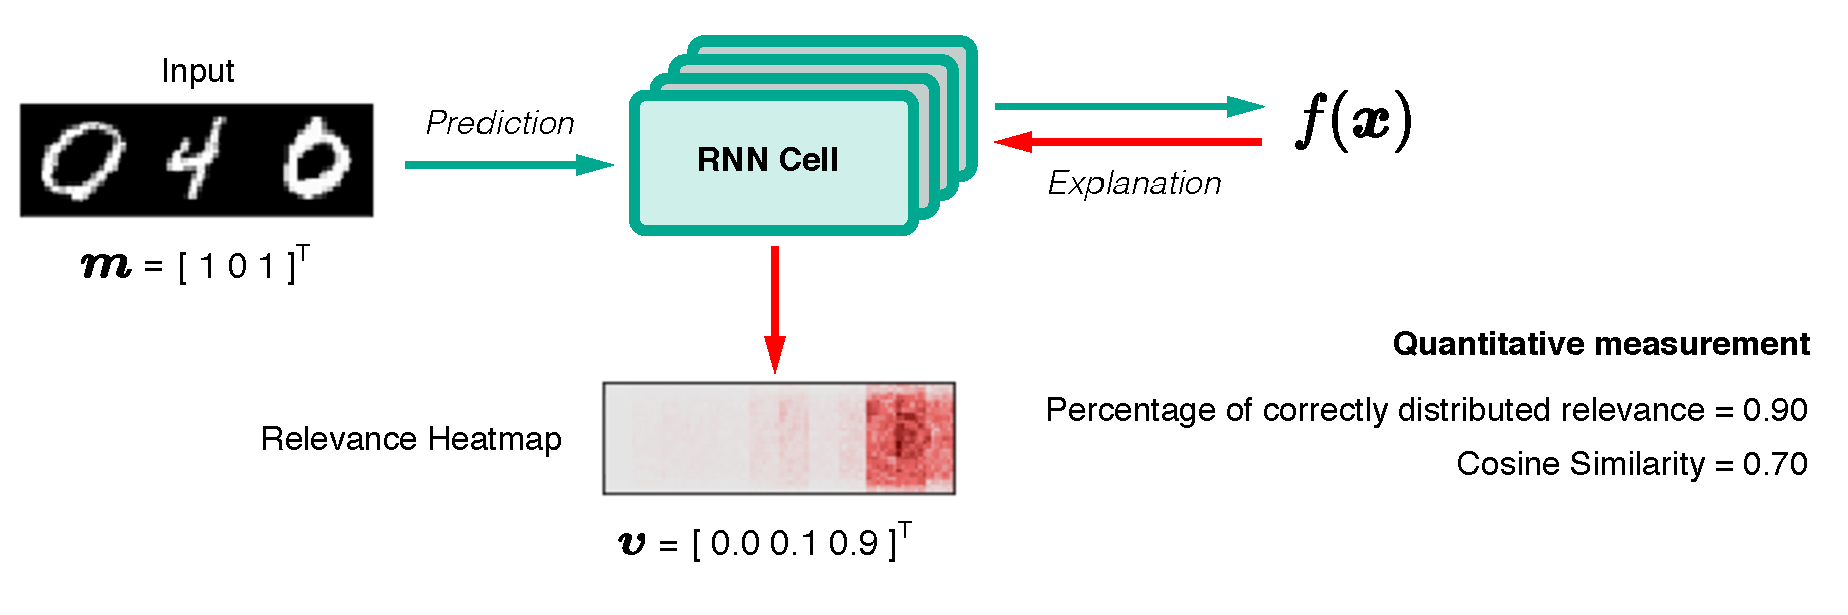
\includegraphics[width=\textwidth]{sketch/quantitative_evaluation}
\patcaption{Comparison of two quantitative measurements:  the percentage of correctly distributed relevance scores and the cosine similarity.}{} 
\label{fig:quantitative_evaluation}
\end{figure}

We conducted quantitative evaluations using $k$-fold cross-validation process. The cross-validation allows us to take into account variations that might be introduced from various sources, such as variable initialization, hence yielding more robust results. We combined original training and testing set together to create $k$ folds cross-validation data. Models were trained on $k-1$ folds. Each fold is used as the testing set once, and the cosine similarity is averaged from test samples.  We choose $k=7$ to preserve the original proportion of the training and testing data.




% todo Statistical Evaluation
%\subsubsection{Statistical Evaluation}
%hypo : check whether we need it: 
%It is also possible that some architectures might perform similarly and the difference is not visually observed. For such scenarios, we will use one-way ANOVA on statistics of cosine similarity and pairwise Tukey Honest Significant Difference (HSD) as a post-hoc test to verify whether there are statistically significant results. We use significance level at $0.05$. Dataset is considered as a confounding variable. This procedure is conducted separately for each explanation method.
%}



 %Table x show accuracy sf

\subsection{Result}

\renewcommand{\arraystretch}{1.5}
\begin{table}[!hbt]
\begin{center}
\begin{tabular}{lc|c|c|}
\cline{3-4}
& &
\multicolumn{2}{c|}{\parbox{3.5cm}{ \vskip 1mm \centering \textbf{Accuracy} \vskip 1mm}} \\ \hline
\multicolumn{1}{|l|}{\textbf{Cell architecture}} & \textbf{No. variables} & \textbf{MNIST-MAJ} & \textbf{FashionMNIST-MAJ} \\ \hline
\multicolumn{1}{|l|}{Shallow}    & 184,330          & 98.12\% & 90.00\% \\ 
\multicolumn{1}{|l|}{Deep}       & 153,578           & 98.16\% & 89.81\% \\ 
 \multicolumn{1}{|l|}{DeepV2}     & 161,386        & 98.26\% & 90.57\% \\
\multicolumn{1}{|l|}{ConvDeep}   & 151,802       & 99.22\% & 92.87\%  \\ \hline 
\end{tabular}

\end{center}
\patcaption{Numbers of trainable variables and model accuracies of the Shallow, Deep, DeepV2, and ConvDeep architectures on MNIST-MAJ and FashionMNIST-MAJ with sequence length $T=12$.}{The accuracies are computed from the test set.}
\label{tab:maj_rnn_model_acc}
\end{table}
\renewcommand{\arraystretch}{1}

 \begin{figure}[!htb]
\centering
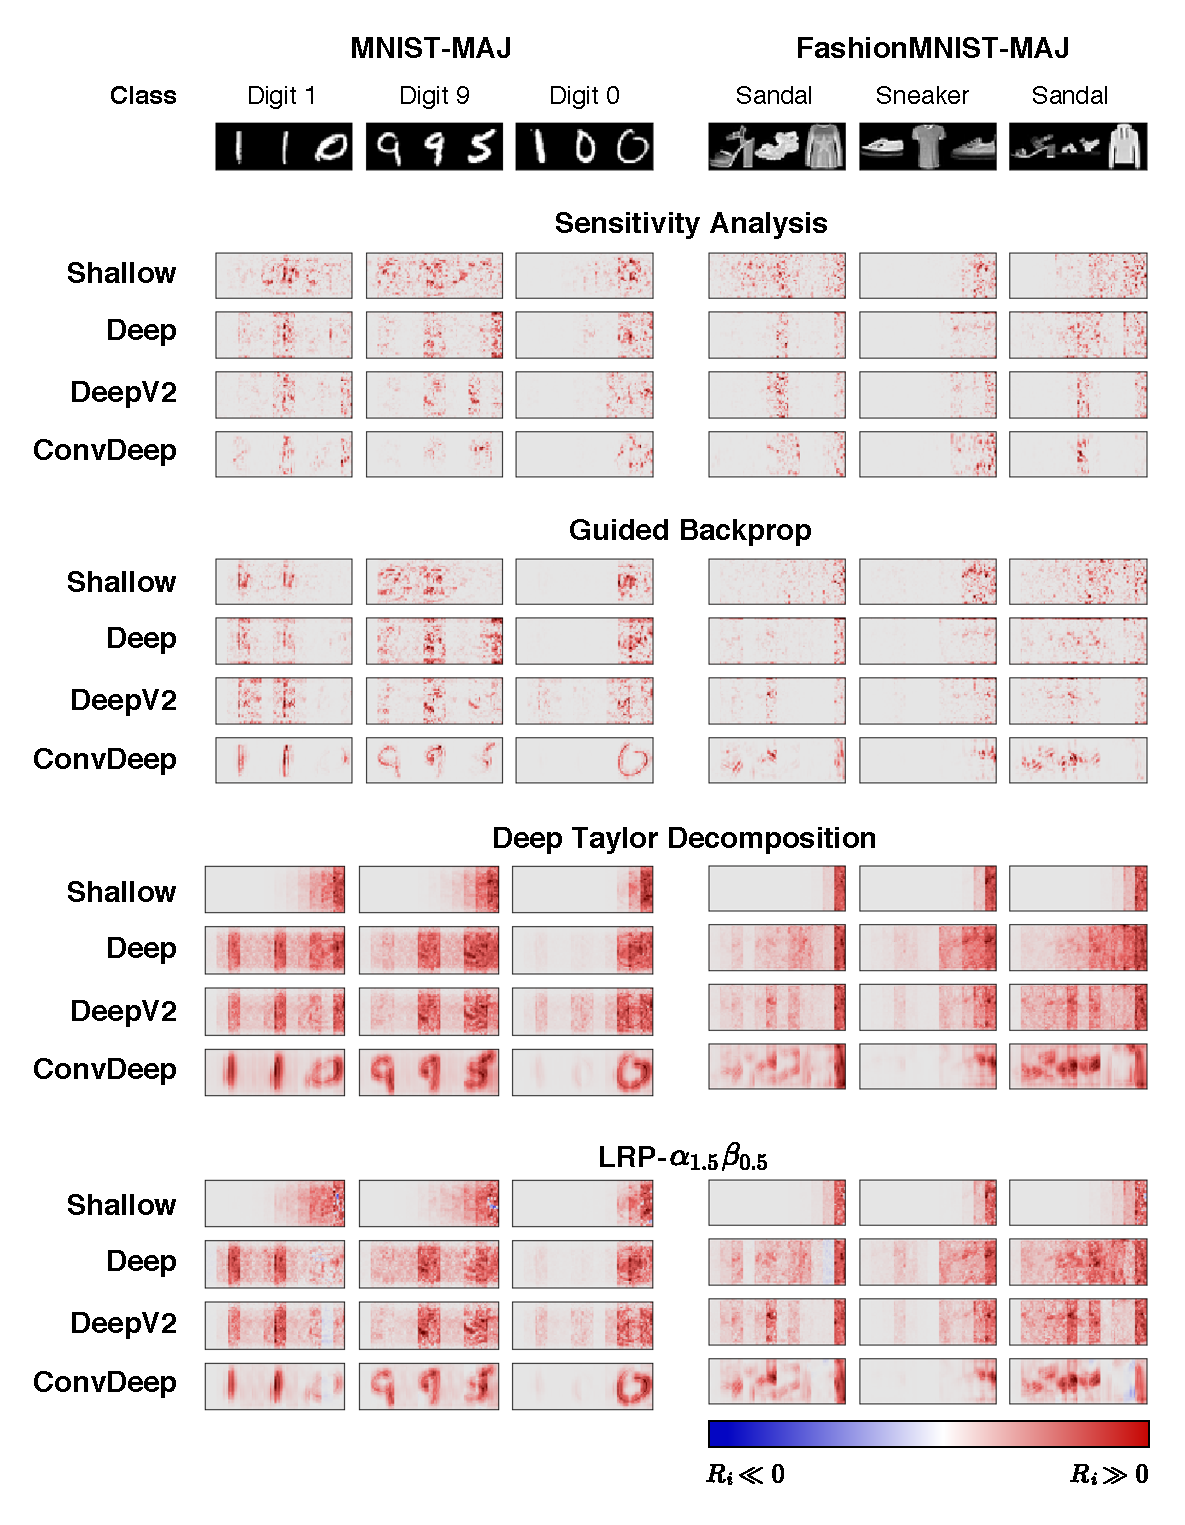
\includegraphics[width=0.8\textwidth]{sketch/heatmap_msc_for_thesis}
\patcaption{Relevance heatmaps from different explanation techniques applied to the Shallow, Deep, DeepV2, and ConvDeep architectures \trainon.}{\heatmapscaleexplain } 
\label{fig:heatmap_msc_mix_for_thesis}
\end{figure}

Table \ref{tab:maj_rnn_model_acc} shows numbers of trainable variables and accuracies of the trained models for qualitative inspections. These trained models have an equivalent number of variables and accuracy, except the ConvDeep architecture that has slightly higher accuracy. \addfigure{\ref{fig:heatmap_msc_mix_for_thesis}} shows that deeper architectures provide higher quality explanations, in other words, their predictions are more explainable. In particular, we can see that the portion of relevant scores distributed to irrelevant region is gradually reduced from the Shallow to ConvDeep architectures. This improvement can be observed on all explanation methods. This result further supports the evidence shown in Section \ref{sec:exp1}.  

Although the explanation heatmaps from the \rnncell{Shallow}, \rnncell{Deep}, and \rnncell{DeepV2} architectures look noisy, increasing the depth of architecture seems to reduce the noise in the heatmaps as well.   On the other hand, the \rnncell{ConvDeep} architecture adequately manages to propagate relevance quantities to the proper $\x_t$. The architecture produces visually sound heatmaps that well present features of $\x$ that are hardly observed in the explanations from the other architectures.  GB, DTD, and $\lrpp$ heatmaps of Digit 1 and Sandal samples are such examples.

 \begin{figure}[!hbt]
\centering
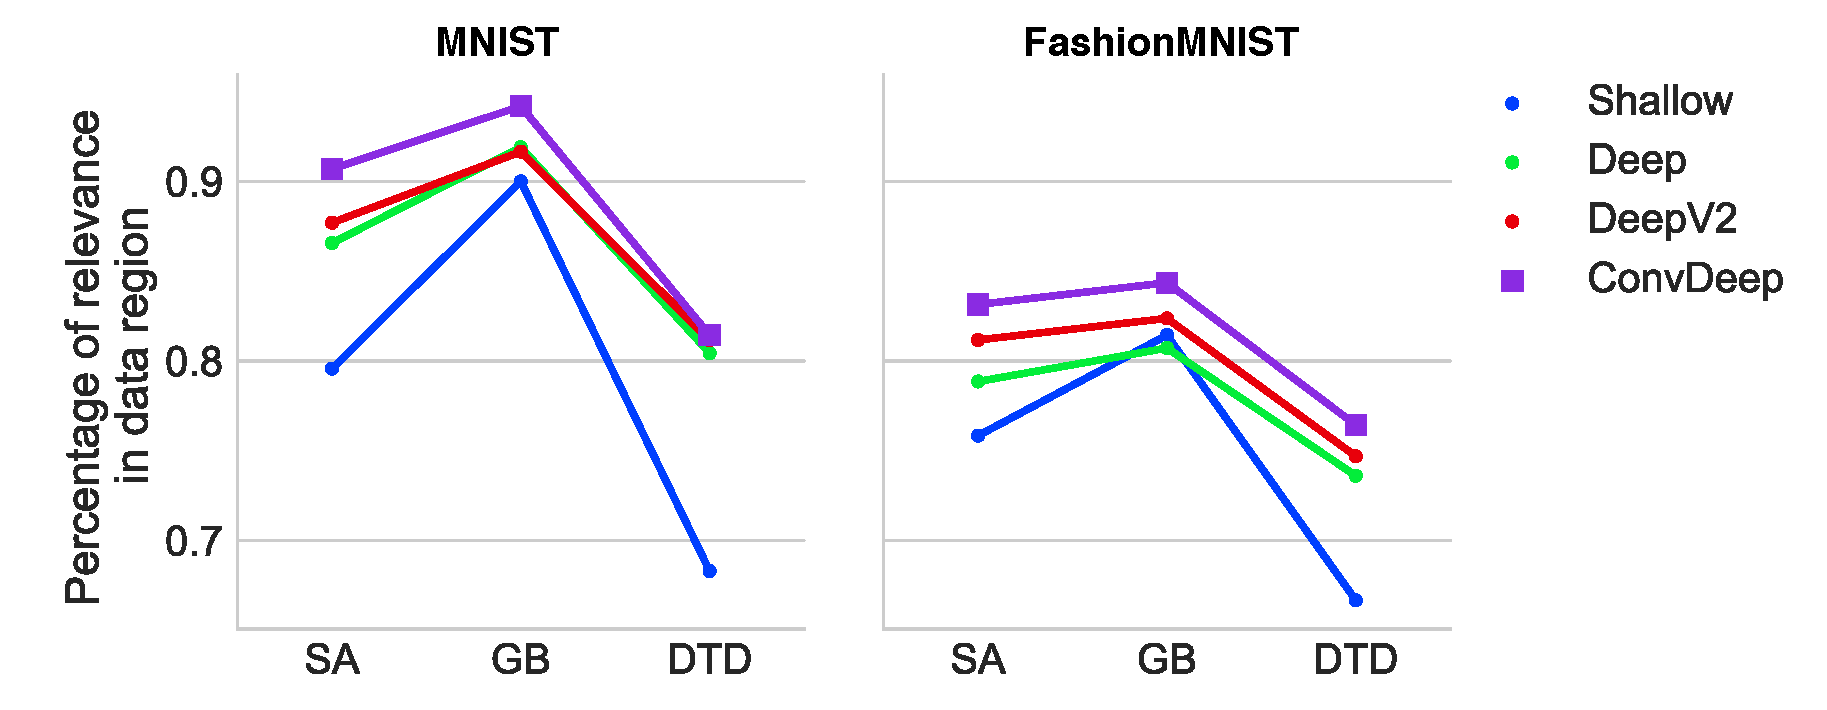
\includegraphics[width=\textwidth]{sketch/rel_dist_maj_3_samples_thesis}

\patcaption{Cosine similarity measurement from different explanation techniques applied to the Shallow, Deep, DeepV2, and ConvDeep architectures \trainon.}{The baseline is the Shallow architecture presented in blue. \quantitativeplotexplain}


\label{fig:rel_dist_maj_3_samples_thesis}
\end{figure}

\addfigure{\ref{fig:rel_dist_maj_3_samples_thesis}} presents quantitive evaluations of the impact from the depth of architecture on the quality of explanation. As a reminder, the measurement is the cosine similarity between the binary vector $\boldsymbol{m} \in \mathbb{R}^3$ and the vector of aggregated relevance scores of $28\times28$ blocks $\boldsymbol{\upsilon} \in \mathbb{R}^3$. The cosine similarity is averaged from test sets of $7$-fold cross-validation procedure as described in Section \ref{sec:evaluation_med}. Results from \addfigure{\ref{fig:rel_dist_maj_3_samples_thesis}} indicate that increasing the depth of architecture indeed improves the quality of explanations. In particular, the averaged cosine similarity of each explanation technique systematically increases when introducing  more layers. This effect can be seen clearly from the result of FashionMNIST-MAJ. Additionally, we can also observe that the difference of the similarity between the baseline architecture, \rnncell{Shallow}, and the other  architectures changes with different proposition across methods. More precisely, we see that the proportional improvement of  DTD and $\lrpp$ are much more substantial than the other methods. This implies that some explanation methods are more sensitive to RNN architecture than the others.


% todo hypo : pair wise statistical testing

\subsection{Summary}
The results of this experiment quantitively confirm that the architecture of RNNs is indeed an essential factor to the explainability of RNN models, especially in the aspect of propagating relevance quantities to corresponding input steps.  The results also show that the impact affects the quality of explanation in different level on different methods. More precisely, DTD and LRP techniques are more sensitive to the architecture of explained models than SA and GB methods.

Nonetheless, we  still observed that there are some samples whose significant amount of relevance scores are distributed to irrelevant regions even using the ConvDeep architecture. The DTD and $\lrpp$ explanations of Digit ``9" in \addfigure{\ref{fig:heatmap_msc_mix_for_thesis}} are such examples. For those heatmaps, relevance scores should not be allocated to the block of ``5".   Therefore, we are going to propose several improvements to mitigate the issue.

